
\documentclass[12pt,a4paper,titlepage,oneside]{report}
%\errorcontextlines=1000
\usepackage{amsfonts}
\usepackage{amsmath}
\usepackage{amsopn}
\usepackage{amssymb}  % ermoeglicht u.a. $\frak{}$
\usepackage{mythm}    % anstelle von amsthm wegen neuem Theoremstil `fact'
\usepackage{amscd}
\usepackage{german}
\usepackage{graphics}
\usepackage[final]{graphicx}
\usepackage{graphpap} % um beim Zeichnen ein Raster zu sehen
\usepackage{ifthen}   % ermoeglicht \ifthenelse{}{}{}
\usepackage{makeidx}
\usepackage{umlaut}  	% Eingabe von Umlauten als ��,�
\usepackage{epic}  	% Enhancement to Picture Environments
\usepackage{psfig}  	% Import von ps/eps-Dateien mit\psfig{file=...}
\usepackage{parskip}  	% statt Einruecken von Abs�zen Zeilenvorschub

\textwidth13.5cm
\hoffset0.2cm
\textheight22.5cm
\voffset-0.5cm
%\parindent0em
%\parskip1ex
\makeindex
\frenchspacing                   % Leerzeichen verschieden breit :-)
\sloppy                          % mehr Trennungen erlauben ...
\hbadness = 10000
\begin{document}

  \bibliographystyle{alpha}      % Stil fuer Literaturzitate
  % \setcounter{tocdepth}{4}     % auf Wunsch bis zu 4 Ebenen im
  % \setcounter{secnumdepth}{4}  % Inhaltsverzeichnis!

  \psfull                       % ps/eps-Dateien wirklich importieren?
  %\psdraft                      % Oder nur die BoundingBox benutzen?
  %\pssilent                     % keine Meldungen ueber ps/eps-Import

  \fboxsep 0mm                   % kein Abstand zwischen Rahmen und Bild?

	\begin{titlepage}
		\large
		\begin{center}
		\begin{figure}[h]
			\begin{center}
			
\includegraphics{pix/TUMs.eps}
			\end{center}
		\end{figure}
		Technische Universit"at M"unchen\\
		\vspace{0.1cm}
		Fakult"at f"ur Mathematik\\
		\vspace{4cm}
		\LARGE
		\textbf{Partikelbasierte Fluidsimulation f"ur\\
				interaktive Anwendungen\\
		}
		\vspace{1.6cm}
		\large
		Diplomarbeit von Leo Wandersleb\\
		\vspace{8.5cm}
		\large
		\begin{tabular}{ll}
		Aufgabensteller: & Prof. Dr. Thomas Huckle\\
		Betreuer: & Prof. Dr. R"udiger Westermann\\
		Abgabetermin: & 17. Januar 2005\\
		\end{tabular}
		\end{center}
	\end{titlepage}
	\pagestyle{empty}
	\cleardoublepage
	\hfill\\
	\vspace{18cm}
	\hfill\\
	\normalsize
	Hiermit erkl"are ich, die Diplomarbeit selbst"andig und nur mit den angegebenen Hilfsmitteln angefertigt zu haben.

	\vspace{1cm}

	M�nchen, den 16. Januar 2005

	\hfill
	(Leo Wandersleb)

	\cleardoublepage
	\begin{abstract}
Wasser zu simulieren ist im Bereich der Computergrafik immer noch eine gro"se Herausforderung.
Auch wenn auf dem Gebiet der Offline-Simulation zunehmend plausible Resultate zu sehen sind, wie z.B. in den Kinofilmen "`Titanic"' (1997), "`Antz"' (1998) oder "`Finding Nemo"' (2003), ist das Simulieren von Fl"ussigkeiten im interaktiven Bereich ein weitgehend unbestelltes Feld.
Dank der erreichten Leistungsst"arke aktueller PCs ist eine solche Simulation mit vern"unftigem Aufwand realisierbar.

In der vorliegenden Arbeit soll der Ansatz von Matthias M"uller, David Charypar \& Markus Gross \cite{ETHZ} fortgef"uhrt werden und durch eine neuartige Datenstruktur der Speicherbedarf bei gleichzeitiger Vergr"o"serung des Simulationsgebiets verringert werden.
W"ahrend das Programm zur vorliegenden Arbeit bei h"oheren Bildraten mit unter 15MB RAM auskommt, konnte das Simulationsgebiet auf das etwa hunderttausendfache gesteigert werden.
\end{abstract}

	\cleardoublepage
	\setcounter{page}{1}           % ab hier Seitennumerierung mit 1
	\pagestyle{plain}

	\tableofcontents
	\cleardoublepage

	\chapter{Einf�hrung}
Obwohl schon viel gearbeitet und geforscht wurde auf dem Gebiet der Fluidsimulation, steckt sie immer noch in den Kinderschuhen.
Insbesondere gibt es noch keine interaktiven Verfahren, die auf gro�en Gebieten Wasser im Raum, also nicht als H"ohenfeld realisieren. Anwendungen hierf�r w�ren etwa Wasserf�lle, Getr�nke oder Wasserwerfer in Computerspielen, aber auch zum Beispiel Blut in Operationssimulatoren.

Den Ansto� zu einem um Gr"o�enordnungen umfangreicheren Simulationsgebiet brachte Herr Prof. Dr. Westermann, als er vorschlug, Zellinformationen nur noch beim Partikel zu speichern und nach diesem Zellindex die Partikel zu sortieren. Durch diese implizite Anordnung der Zellen wird erreicht, dass der Speicherbedarf unabh"angig von der Gr��e des simulierten Gebiets wird und meine Software keine 15MB ben�tigt, um 3000 Partikel in einem Gebiet bestehend aus $(100.000)^3$ Zellen zu simulieren. M�chte man 500.000 Partikel verwenden, so stehen immernoch $(16.000)^3$ Zellen zur Verf�gung.

Laut Nick Fosters \& Ronald Fedkiws {\em "`Practical animation of liquids"'} \cite{FOFE} wurde z.B. f�r die Simulation der Schlammdusche von Dreamworks "`Shrek"' lediglich ein Gitter von 150 x 200 x 150 Zellen verwendet.
Um auf meiner Datenstruktur Physik berechnen zu k"onnen und vor allem um die zugeh"orige Oberfl"ache zu konstruieren, sind allerdings sehr spezialisierte Ans"atze gefragt.
So orientiert sich diese Arbeit im Groben an \cite{ETHZ} von Matthias M"uller, David Charypar \& Markus Gross, passt deren Ans"atze aber auf die erw"ahnte Datenstruktur an.
Au"serdem wird die auf ATI-Grafikkarten vorhandene TRUFORM$^\texttt{TM}$-Erweiterung genutzt, um auf einem relativ groben Gitter mittels des Marching Cube Algorithmus erzeugte, durch ebene Teilfl"achen charakterisierte, also eckige,
Oberfl"achen rund darzustellen.

\section{Zweck und Aufbau dieser Diplomarbeit}
W�hrend urspr�nglich geplant war, aus den Ergebnissen aus \cite{ETHZ} und \cite{UTAH} eine interaktive Simulation f�r Fl�ssigkeiten mit verschiedenen Eigenschaften zu entwickeln, entstanden aus der "`entdeckten"' Methode zur Kollisionsdetektion ganz neue Anforderungen und die Physik trat zun�chst in den Hintergrund.
Au�erdem hat diese Arbeit m"oglicherweise auch Relevanz f�r astronomische Simulationen, wof�r die Methoden der Smoothed Particle Hydrodynamics (SPH) urspr�nglich entwickelt wurden, da hier Verfahren aufgezeigt werden, die den Simulationsbereich herk�mmlicher Anwendungen um Gr��enordnungen �bersteigen.

So werden in Kapitel \ref{Physik} die physikalischen Grundlagen erarbeitet, sowie die Smoothed Particle Hydrodynamic als Methode zur numerischen L�sung von Flussproblemen vorgestellt. In Kapitel \ref{KOL} wird auf die f�r SPH ben�tigte Kollisionsdetektion eingegangen und ein neues Verfahren eingef�hrt. In Kapitel \ref{vis} werden Methoden zur schnellen Oberfl�chenerzeugung entwickelt. Kapitel \ref{anwendung} stellt ein kleines Demonstrationsprogramm vor, welches sich auch auf der beigef�gten CD befindet. In Kapitel \ref{resultate} sind einige Screenshots, so wie Angaben zur Performance zu finden. Kapitel \ref{ausblick} gibt schlie�lich einen Ausblick auf Anwendungsm�glichkeiten und Entwicklungspotential.
	\chapter{Physikalische Grundlagen}
\label{Physik}
Grunds"atzlich gibt es zwei Ans�tze, Physik von Wasser zu berechnen.
\begin{itemize}
	\item Auf einem festen Gitter, was sich empfiehlt, wenn im Wesentlichen alle Gitterpunkte innerhalb des simulierten Mediums sind, also zum Ergebnis beitragen.
	\item Auf Punkten, die sich mit dem Geschwindigkeitsfeld mit bewegen ({\sc Lagrange}'scher Formalismus), was vorzuziehen ist, wenn die Verteilung des Mediums im Raum nicht a priori bekannt ist bzw. sehr stark variiert (Spritzeffekte, Regen, ...).
\end{itemize}

Doch bevor hierauf n�her eingegangen wird, werden Gleichungen ben�tigt, die Fluiddynamik beschreiben.

\section{{\sc Navier-Stokes-}Gleichungen}
Schon Anfang des 19ten Jahrhunderts entwickelten der Franzose Navier und der Brite Stokes ein Gleichungssystem, um das Verhalten von Fl�ssigkeiten zu beschreiben. Dabei werden Viskosit�t, Druck, K�rperkr�fte sowie Massen- und Impulserhaltung ber�cksichtigt.

Die Viskosit�tskraft
\begin{equation*}
	\label{visc}
	\frac{\vec{F}_{\mbox{Viskosit�t}}}{V} = \eta \nabla ^2 \vec{v},
\end{equation*}
die proportional zur Viskosit�t  $\eta$ in Richtung der Geschwindigkeits�nderung wirkt, die Druckkraft
\begin{equation*}
	\label{druck}
	\frac{\vec{F}_{\mbox{Druck}}}{V} = - \nabla P,
\end{equation*}
die entgegen dem Druckgradienten, also in Richtung des gr��ten Druckabfalls wirkt, und eine sogenannte K�rperkraft
\begin{equation*}
	\label{aussen}
	\frac{\vec{F}_{\mbox{K�rper}}}{V} = F,
\end{equation*}
wie zum Beispiel die Gravitationskraft ergeben mit dem Impuls $\vec{p}$ und
\begin{equation*}
	\label{newton}
	\frac{\vec{F}}{V} = \frac{1}{V}\frac{d\vec{p}}{dt} = \rho \frac{D\vec{v}}{Dt} = \rho \frac{\partial\vec{v}}{\partial t} + \rho \vec{v} \cdot \nabla \vec{v}
\end{equation*}
(Newtons Gesetz der Fluiddynamik) die Gleichung
\begin{equation*}
	\rho\frac{\partial\vec{v}}{\partial t} + \rho \vec{v} \cdot \nabla \vec{v} = F - \nabla p + \eta \nabla^2 \vec{v}.
\end{equation*}
Teilt man nun durch $\rho$, so erh�lt man
\begin{equation}
	\label{ns1}
	\frac{\partial\vec{v}}{\partial t} + \vec{v} \cdot \nabla \vec{v} = \frac{F}{\rho} - \frac{\nabla p}{\rho} + \nu \nabla^2 \vec{v},
\end{equation}
wobei $\nu = \frac{\eta}{\rho}$ als kinematische Viskosit�t bezeichnet wird.

Gleichung \ref{ns1} und die Kontinuit�tsgleichung
\begin{equation}
	\label{ns2}
	\frac{\partial \rho}{\partial t} =
		- \nabla (\rho \cdot \vec{v}) =
		- \vec{v} \cdot \underbrace{\nabla \rho}_{=0} - \rho \nabla \cdot \vec{v} = - \rho \nabla \cdot \vec{v}
\end{equation}
werden zusammen als {\sc Navier-Stokes}-Gleichungen bezeichnet.

Die Kontinuit�tsgleichung unter Annahme der Inkompressibilit�t (Gleichung \ref{ns2}) beschreibt in Worten, dass die �nderung der Dichte proportional zum Negativen der Divergenz des Geschwindigkeitsfeldes, also zum Zufluss ist. Ein positiver Zufluss bedeutet ein Steigen der Dichte.

Diese Einf�hrung zu den {\sc Navier-Stokes} Gleichungen und weiterf�hrende Links finden sich bei \cite{NSG}.

Die vorliegende Arbeit verwendet den {\sc Lagrange}'schen Formalismus, wodurch sich, wie in \cite{ETHZ} beschrieben, einige Vereinfachungen ergeben. So kann die f�r den Massenerhalt zust�ndige Gleichung \ref{ns2} ganz weggelassen werden, da die Masse auf Partikeln gespeichert ohnehin konstant bleibt.

Da sich die Partikel mit der Fl�ssigkeit bewegen, wird auch der konvektive Term aus Gleichung \ref{ns1} nicht ben�tigt, und die linke Seite von Gleichung \ref{ns1} ist nur noch die Zeitableitung der Geschwindigkeit $d\vec{v}/d t$. Mit der Kraft
\begin{equation}
	\label{einfach}
	f = F - \nabla p + \nu \nabla^2 \vec{v}
\end{equation}
ergibt sich als Beschleunigung $\vec{a}$ f�r das $i$-te Partikel
\begin{equation}
	\label{nspar}
	\vec{a}_i = \frac{d\vec{v}_i}{dt}=\frac{f_i}{\rho_i}.
\end{equation}
Um diese Gleichungen aber numerisch zu l�sen, also insbesondere die physikalischen Gr��en im Raum zu bestimmen, wird hier Smoothed Particle Hydrodynamics (SPH) verwendet.

\section{Smoothed Particle Hydrodynamics}
\label{SPH}

Im SPH-Formalismus wird die Verteilung einer physikalischen Gr��e $u$ im Raum durch Gl�tten der auf Partikelpositionen gespeicherten Werte $\langle u \rangle$ approximiert.
\begin{equation*}
	\label{smoothing}
	\langle u (\vec{x})\rangle = \int_V u(\vec{x})W(\vec{x}-\vec{x}',h)dV
\end{equation*}

Dabei muss der Gl�ttungskern $W(\vec{x}-\vec{x}',h)$ normiert sein, also
\begin{equation}
	\label{eq:normiert}
	\int_V W(\vec{x}-\vec{x}',h) dV = 1
\end{equation}
gelten, und unter Verwendung einer Gl�ttungsl�nge $h \rightarrow 0$ muss der gegl�ttete Wert $\langle u (\vec{x})\rangle$ gegen $u (\vec{x})$ gehen.
\begin{equation}
	\label{eq:limit}
	h \rightarrow 0 \Rightarrow \langle u (\vec{x})\rangle \rightarrow u (\vec{x})
\end{equation}
\paragraph{Notation:}In sp�teren Kapiteln ist von {\em Partikelradius}, {\em Interaktionsradius} oder kurz {\em Radius} die Rede. Damit ist immer die dann f�r alle Partikel und Gl�ttungskerne konstante {\em Gl�ttungsl�nge} gemeint.

Mit Hilfe dieser Gl�ttungskerne kann nun $u$ an jedem Punkt im Raum als Summe �ber alle gegl�tteten Partikel bestimmt werden.
Dieser Wert ist im Allgemeinen nicht exakt, aber Olaf Kessel-Deynet zeigt in \cite{SPH}, dass es schon gen�gt, zus�tzlich zu den Gleichungen \ref{eq:normiert} und \ref{eq:limit} zu verlangen, dass $W$ gerade ($W(\vec{x},h)=W(-\vec{x},h)$) ist, um eine in $h$ quadratische Fehlerordnung zu erhalten.

\begin{equation*}
	\langle u(\vec{x}) \rangle = \sum_i \frac{m_i}{\rho(\vec{x}_i)} u(\vec{x}_i) W(\vert\vec{x}-\vec{x}_i\vert, h),
\end{equation*}

wobei $m_i, \rho(\vec{x}_i)$ und $u(\vec{x}_i)$ die entsprechenden Gr��en am $i$-ten SPH-Partikel sind.

SPH ist durch die M�glichkeit der freien Platzierung von Partikeln im Simulationsgebiet speziell geeignet, Prozesse, die sich auf einem komplizierten r�umlichen Gebiet abspielen, zu simulieren, da die Partikel zum Zweck erh"ohter Genauigkeit in relevanten Bereichen lokal dichter und in anderen, die nur geringen oder gar keinen Einfluss auf die Simulation haben, auch gar nicht platziert werden k�nnen.
Auch ist eine Neuplatzierung dieser Partikel f�r jeden Zeitschritt meist sinnvoll. So eben auch bei der Simulation von Wasser. In meiner Arbeit transportiere ich die Partikelposition schlicht mit der Geschwindigkeit des Wassers. Andere Ans�tze, die dies lediglich als erste Approximation w�hlen, werden zum Beispiel in \cite{UTAH} verwendet.

In dieser Arbeit wird das Gleichungssystem \ref{nspar} gel�st, indem in einem ersten Durchlauf f�r jedes Partikel die Dichte $\rho$ als Summe der gegl�tteten Dichten aller Partikel bestimmt wird und in einem zweiten Durchlauf die von $\rho$ abh�ngigen gegl�tteten Kr�fte aufsummiert werden. Da die Gl�ttungsl�nge $h$ klein ist, muss nicht �ber alle Partikel summiert werden, sondern nur �ber Partikel in der jeweiligen $h$-Umgebung. Um das zu optimieren, wird eine effiziente Kollisionsdetektion ben�tigt.
	\chapter{Kollisionsdetektion}
\label{KOL}
Da der Aufwand f"ur die $n$-Partikel-Kollisionsdetektion die Ordnung $n^2$ h�tte (jedes Partikel kommt f�r jedes andere Partikel als Kollisionspartner in Frage), ist es notwendig, sich hier�ber Gedanken zu machen. Um ein plausibles Ergebnis der Fl�ssigkeitsbewegung zu erhalten, gen�gt es, wie in \ref{SPH} beschrieben, die Physik in jedem Punkt der {\sc Lagrange}'schen Simulation (Partikel) nur auf einem kompakten Tr�ger zu berechnen. Der Radius dieses Tr�gers bestimmt ma�geblich die Komplexit�t der Simulation.
Da die Partikel keinen Einflu"s auf das gesamte Gebiet haben, sondern nur auf ihre unmittelbare Umgebung, empfiehlt sich nun eine Raumpartitionierung.
Es wird nur der Abstand zu den Partikeln ermittelt, deren Raumpartition sich mit dem Tr"ager der physikalischen Gr"o"sen des betrachteten Partikels schneidet.
Dadurch wird der Aufwand von $n^2$ auf $\sum_{i=1}^n k_i^2 \le k*n$ \label{coll_ord} reduziert, wobei $k_i$ die Anzahl der Partikel in der Partition des $i$-ten Partikels und $k$ die maximale Anzahl an Partikeln pro Raumpartition ist. Nimmt man den Bereich $B_r$ jedes Partikels als Raumpartition, so erh�lt man das von der Physik abh�ngige optimale $k^{opt}$.
Damit ist $k$ ein Ma� daf�r, zu wie vielen Partikeln der Abstand berechnet werden muss. Also gibt $k / k^{opt}$ an, wie viele Abst�nde zu viel gemessen werden, was insbesondere dann eine gro�e Rolle spielt, wenn die Physik bei einer Kollision sehr billig zu berechnen, die Ermittlung des Abstandes jedoch schon vergleichbar teuer ist.

\section{Explizite Raumpartitionierung}
In einem ersten Schritt erprobte ich die Kollisionsdetektion mittels expliziter Speicherung der Partikelindizes pro Raumpartition mit einem regelm"a"sigen Gitter als Raumpartitionierung. Also etwa $200^3$ Zellen mit der M"oglichkeit, pro Zelle 20 Partikelindizes zu speichern. Dies setzt voraus, dass die Physik niemals mehr als 20 Partikel pro Zelle zul�sst. Unter Verwendung von vier Byte Adressen f�r die Partikel resultierte das in einem Speicherbedarf zu Programmstart von $200^3*20*4$B$=640$MB.

Der auf diesem Gitter arbeitende Algorithmus musste entweder berechnen, mit welcher der benachbarten 26 Zellen das Partikel interagieren kann ($20 \le k \le 8*20 = 160$), oder man durchsucht pauschal alle 27 Zellen, die das Partikel enthalten bzw. die das Partikel enthaltende Zelle umgeben ($k = 27*20 = 540$). Zweiteres ist wohl das Praktikablere, da hier mit einer Zellkantenl�nge $\approx r$ der Wert $k$ sehr nahe $k^{opt}$ ist. Ersteres macht nur Sinn, wenn die Zellkantenl�nge $\ll r$ ist, was wiederum bedeuten w�rde, dass mit 20 Partikeln pro Zelle nur wenige dieser Partikel interagieren k�nnen.

Eine dynamische Speicherbelegung reduzierte zwar den Speicherbedarf auf 1B pro Zelle f"ur leere Zellen, was mir allerdings zum einen nicht die schon angek"undigten mehr als $10.000^3$ Zellen ($\hat{=} 10.000^3$B$ = 1$TB) erm"oglicht, zum anderen f"ur manche Situationen, wie etwa Regen, den Aufwand f"ur \emph{Speicher freigeben} und \emph{Speicher reservieren}
extrem in die H�he treibt.

\paragraph{Exkurs (Jedem Partikel seine Zelle):}
\label{vieleGitter}
Um nur die Partikel einer Zelle auf Abstand $d < r_0$ pr"ufen zu m"ussen, k�nnen auch verschobene regul"are Gitter der Kantenl"ange $4r_0$ erzeugt werden.

Eindimensional ben"otigt man zwei Gitter:
\begin{itemize}
	\item {Gitter $g=0$:}		$\left\{ \left[j(4r_0); (j+1)(4r_0)\right[ | j\in
		\texttt{N}\right\}$
	\item {Gitter $g=1$:}		$\left\{ \left[(j+\frac{1}{2})(4r_0); (j+\frac{3}{2})(4r_0)
		\right] | j\in \texttt{N}\right\}$
\end{itemize}
Als Kollisionspartner f"ur ein Partikel an Position $x$ kommen nur
Partikel in Zelle $(g, j)$ mit
\begin{eqnarray*}
g&=&\left|\left(\frac{x}{4r_0} - \left\lfloor \frac{x}{4r_0}\right\rfloor
\right)*4-2\right|\cr
j&=&\frac{x-2gr_0}{4r_0}
\end{eqnarray*}
in Frage.

Im Zweidimensionalen werden vier und im Dreidimensionalen gar 8 Gitter ben"otigt. Zur Veranschaulichung des zweidimensionalen Falls dient Abb. \ref{fig:movingparticleingrid} auf Seite \pageref{fig:movingparticleingrid}.

Mir ist keine Implementierungen dieser vielen Gitter bekannt, wohl auch, da ein begrenzender Faktor der Speicherplatz ist, der bei einer expliziten Speicherung aller Zellen im Simulationsgebiet eine Verachtfachung\\
(640MB*8=5,12GB) des Speicherbedarfs bedeutet. Deshalb wird in den angrenzenden Zellen in \emph{einem} festen Gitter gesucht.
\section{Implizite Raumpartitionierung}
\label{datenstruktur}Um diesen gigantischen Speicherbedarf zu vermeiden, schlug Herr Prof. Dr. R"udiger Westermann vor, zwar diesen Weg der vielen Gitter zu gehen, die Gitterinformation aber nur bei den Partikeln zu speichern, diese zu sortieren und dadurch in einer Zelle befindliche Partikel zu identifizieren. Bekannte Sortieralgorithmen haben zwar bei $n$ Elementen eine Laufzeitordnung von $n\log n$. Das ist aber gerade im interaktiven Bereich auf Grund der hohen Kosten f"ur die Physik, die wie in \ref{coll_ord} gezeigt eine Ordnung von $kn$ haben, vernachl"assigbar. Beispiell"aufe zeigen, da� selbst bei 1 Mio. Partikeln keine 10\% der Rechenzeit f"ur Sortieren verwendet werden.
In \ref{vieleGitter} habe ich zwar behauptet, man br�uchte im Dreidimensionalen 8 Gittersysteme um garantieren zu k�nnen, dass sich alle Kollisionspartner eines Partikels in einer wie oben bestimmten Zelle befinden.
Was aber unter \ref{vieleGitter} nur eine theoretische �berlegung war, ist bei der impliziten Zelleinteilung Notwendigkeit. In einer Sortierung des $\pmb{R}^3$ kann es nur in zwei Richtungen Nachbarn geben. Die Zellen in der n�chsten Ebene liegen in der sortierten Liste in unbekannter Ferne. Wenn aber diese zwei Richtungen, in denen man die Nachbarzelle finden kann, ausgenutzt werden, so braucht man im $\pmb{R}^3$ nur noch vier Listen.

Im Eindimensionalen wird sofort klar, dass man kein Gitter braucht. Man muss die nach der Koordinate sortierte Liste vom betrachteten Partikel aus nur so lange in beide Richtungen durchlaufen, bis man auf ein Partikel trifft, das zu weit weg ist, um zu kollidieren. Alle Weiteren in dieser Richtung k�nnen nur noch weiter weg sein.

Um im H�herdimensionalen sortieren zu k�nnen, wird ein etwas komplizierteres Kriterium ben�tigt. Hier ist dies ein Zellindex, der sich bei mir wie folgt zusammensetzt:

Die h�chsten Bits repr�sentieren die Position in $z$-Richtung, danach kommt die Position in $y$-Richtung und danach die in $x$-Richtung jeweils als Vielfaches der gew�hlten Zellgr��e (deren Kantenl�nge), die in meiner Software mit $4r$ minimal gew�hlt wurde.

\begin{figure}[htb]
	\begin{center}
	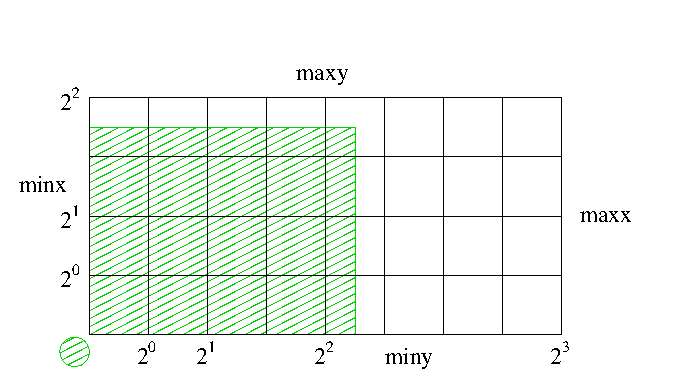
\includegraphics{pix/grid2d.eps}
	\caption{Dieses Gittersystem wird erzeugt, wenn der Benutzer einen Simulationsbereich und einen Interaktionsradius (gr�n) vorgibt.}
	\label{fig:grid2d}
	\end{center}
\end{figure}

Abb. \ref{fig:grid2d} zeigt in 2D, welches Simulationsgebiet bei der Wahl des gr�n schraffierten Gebietes und der gr�n schraffierten Partikelgr��e zur Verf�gung steht. Aus der Bit-weisen Einteilung des Zellindex ergibt sich, dass das Simulationsgebiet in jeder Raumdimension separat auf die Zweierpotenz $*4r$ vergr��ert wird, die gr��er oder gleich der vorgegebenen Abmessung ist.

\paragraph{Exkurs:} Da der Zellindex modulo der �ber die Gr��e des Simulationsgebiets gew�hlten Zellanzahl in der jeweiligen Richtung ermittelt wird, werden Partikeln, die sich au�erhalb des eigentlichen Simulationsgebiets bewegen, ebenfalls "`sinnvolle"' Zellindizes zugeordnet. Viele Aspekte der Simulation sind damit tats�chlich unabh�ngig von der Gr��e des Simulationsgebiets. Insbesondere funktionieren weiterhin alle Partikelinteraktionen, solange der  euklidische Abstand gemessen wird.
Es entsteht lediglich der Mehraufwand der Abstandsmessung zu Partikeln, die sich eine Kantenl�nge des Simulationsgebiets $\pm r$ entfernt befinden, also ohne r�umliche N�he den selben Zellindex erhalten.

Auf diese Weise liegen zwar Partikel aus in $x$-Richtung benachbarten Zellen in der sortierten Liste nahe beieinander, nicht aber Partikel, die in $y$- oder $z$-Richtung in benachbarten Zellen liegen. In diesem Fall k�nnen tausende oder auch nur wenige Partikel zwischen dem betrachteten und dem benachbarten Partikel liegen. Um also alle Kollisionen aufl�sen zu k�nnen, werden Zellen ben�tigt, die genau diese Grenzen abdecken.

\begin{figure}[htb]
	\begin{center}
	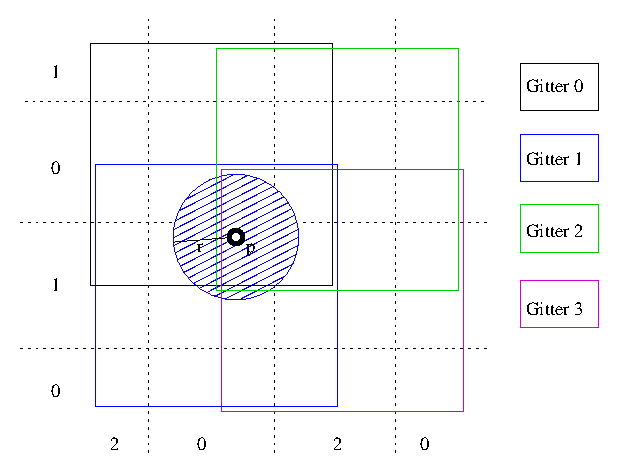
\includegraphics{pix/movingparticleingrid.eps}
	\caption{Dem Partikel zugeordnete Zellen in den vier Gittern mit Zuordnung des relevanten Gitters aus verfeinertem Gitterindex.}
	\label{fig:movingparticleingrid}
	\end{center}
\end{figure}
Abb. \ref{fig:movingparticleingrid} zeigt die eindeutige Zuordnung jeder Position im Raum zu dem Gitter, in dem die zugeh�rige Zelle den Interaktionsbereich eines Partikels komplett umschreibt. Der Gitterindex ist die Summe der am Rand notierten Zahlen. Diese Zahlen werden beim Ermitteln der vier Zellindizes mittels einer zwei Bit feineren Zellindexbestimmung mit ermittelt und direkt als Gitterindex beim Partikel gespeichert.

Um nun alle Kollisionen auszuwerten, werden alle Fl�ssigkeitspartikel durchlaufen, jeweils die relevante Sortierung ausgelesen und in der gew�hlten sortierten Liste so viele nachfolgende und vorhergehende Partikel betrachtet, wie diese einen noch relevanten Zellindex besitzen. Da in $x$-Richtung zwei Bit mehr gespeichert werden, ist der Bereich, �ber den gesucht wird, nicht $4r$, sondern nur $3r$ (siehe Abb. \ref{fig:x2bitplus}). N�mlich die aktuelle $x$-Zelle, der Nachfolger und der Vorg�nger.
\begin{figure}[htb]
	\begin{center}
	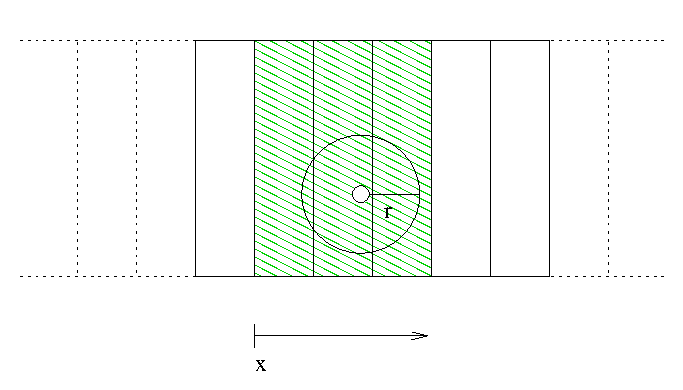
\includegraphics{pix/x2bitplus.eps}
	\caption{In $x$-Richtung wird eine feinere Zellunterteilung verwendet.}
	\label{fig:x2bitplus}
	\end{center}
\end{figure}

Hier lie�e sich durch das Verwenden weiterer Bits eine noch feinere Unterteilung realisieren.
\begin{eqnarray*}
	\mbox{Bit} & \mbox{Gr��e} & \mbox{Verwendung bei}\\
	1 & 4r & y,z\\
	2 & 3r & x\\
	3 & 2\frac{1}{2}r &\\
	4 & 2\frac{1}{4}r &\\
	5 & 2\frac{1}{8}r &\\
	  & \dots &
\end{eqnarray*}
In meiner Anwendung ist eine Verwendung nicht ben�tigter Bits zu diesem Zweck nicht vorgesehen.

Da alle Kr�fte symmetrisch sind, gen�gt es, bei beiden Kollisionspartnern die inversen Kr�fte zu addieren. Um also nicht a mit b und b mit a kollidieren zu lassen, wird jetzt gepr�ft, ob der Index des Kollisionspartners gr��er ist als der des aktuellen Partikels. Ist dies der Fall, so wird die eigentliche Interaktion der Partikel berechnet. Um Kontrolle �ber das Verhalten der Fl�ssigkeit zu erlangen, verwende ich neben den SPH-Partikeln auch spezielle Partikel, die direkte Ver�nderungen an den SPH-Partikeleigenschaften bewirken. Diese haben immer einen h�heren Index als SPH-Partikel. N�heres dazu in Kapitel \ref{Kontrollpartikel} und \ref{trianglelist2boundary}.

Der Kollisionspartner kann also entweder selbst ein Fl�ssigkeitspartikel oder ein Kontrollpartikel sein.
\subsection{Fl�ssigkeitspartikel}
\label{Fluessigkeitspartikel}
Fl�ssigkeitspartikel kommen als Kollisionspartner in Frage, wenn der Abstand kleiner als $r$ ist. Das hei�t, es muss der Abstand zu dem wie eben beschrieben gefundenen Partikel gemessen werden. Ist dieser kleiner als $r$, so wird Fl�ssigkeitsphysik wie in Kapitel \ref{Physik} beschrieben angewendet.
\subsection{Kontrollpartikel}
\label{Kontrollpartikel}
Um m�glichst wenige Kontrollpartikel zu ben�tigen, wird hier die Tatsache ausgen�tzt, dass nach
\begin{equation*}
	V_{\mbox{Zelle}}/\mbox{Kollisionsvolumen}=4r*4r*3r /(\frac{4}{3} \pi r^3)=\frac{36}{\pi}
\end{equation*}
etwa $11.46$ mal so viel Raum nach potentiellen Kollisionspartnern durchsucht wird, wie f�r die Physik �berhaupt in Frage kommt. Bei der Kollision mit Kontrollpartikeln wird kein Partikelabstand gemessen, sondern der Abstand zur Kontrollpartikelebene (siehe Abb. \ref{fig:controllparticleingrid}). Ist dieser negativ, so tritt das Kontrollpartikel in Aktion. Wie in Abb. \ref{fig:controllparticle3d} dargestellt, wird der positive Abstand durch die Orientierung des Dreiecks bestimmt, das zur Initialisirung des Kontrollpartikels verwendet wurde.

\paragraph{Bemerkung:} Solange Kontrollpartikel sich nicht bewegen, k�nnten sie auch einmal vorsortiert werden, um sie dann in einem Schritt eines Merge-Sort-Algorithmus mit der sortierten Liste der bewegten Partikel zu kombinieren. Dadurch w�re die Laufzeitordnung der Sortierung nurnoch in der Anzahl der bewegten Partikel $n\log(n)$ und linear in der Anzahl der Kontrollpartikel.

\begin{figure}[htb]
	\begin{center}
	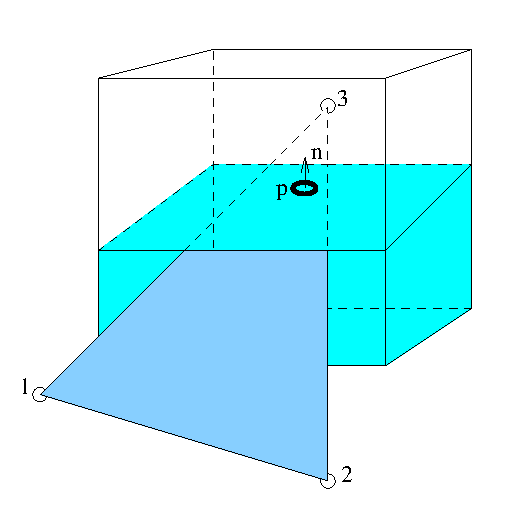
\includegraphics{pix/controllparticle3d.eps}
	\caption{Die Orientierung des verwendeten Dreiecks bestimmt die Normalenrichtung.}
	\label{fig:controllparticle3d}
	\end{center}
\end{figure}
\begin{figure}[htpb]
	\begin{center}
	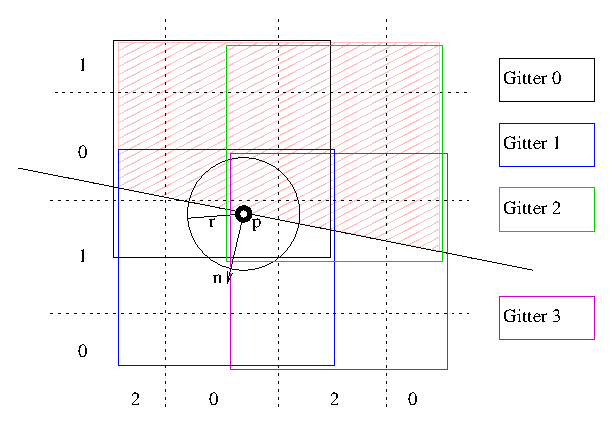
\includegraphics{pix/controllparticleingrid.eps}
	\caption{Lage des Kontrollpartikels in Verh�ltnis zum betroffenen Bereich.}
	\label{fig:controllparticleingrid}
	\end{center}
\end{figure}
	\chapter{Visualisierung}
\label{vis}
Zur Visualisierung w"ahle ich ausschlie"slich eine Art Marching-Cube Verfahren (MCA, siehe \cite{MC}). Anfangs lie� ich diesen Marching Cube (MC) auf der selben Gitterstruktur laufen wie die Kollisionsdetektion. Das erwies sich aber aus verschiedenen Gr�nden als nicht optimal. Die auf diese Weise konstruierte H�lle war zu eckig und die Bewegungen zu sprunghaft, da ja nur diskrete Gitterpositionen zur Verf�gung standen. Mit den folgenden drei Ans�tzen konnten einige Probleme behoben werden.
\begin{itemize}
	\item {Fl�chen h�herer Ordnung}\\
		Da der MCA als kleinste Einheit Oktaeder erzeugt und diese durch einzelne herumfliegende Partikel sehr h�ufig zu Stande kommen, eignet er sich a priori nicht, auch nur ann�hernd runde Formen zu generieren. Diesem Problem konnte ich dank ATI-TRUFORM mit einer k�nstlichen Verfeinerung der Triangulierung mittels der Normaleninformation in jedem Vertex beikommen.
	\item {Deformiertes Gitter}\\
		Um den Spr�ngen von einer Gitterkoordinaten zur n�chsten Herr zu werden, f�hrte ich eine Verformung des MC-Gitters ein, die es insbesondere erlaubt, einzelne Tr�pfchen darzustellen, ohne dass man eine Gitterstruktur erkennt.
	\item {Verfeinertes Gitter}\\
		Meine Ans�tze, das Gitter zu verfeinern, haben leider nicht den gro�en Erfolg gebracht, da die unangenehmsten Artefakte des MCA nicht beseitigt werden konnten.
\end{itemize}
\section{Der Marching Cube Algorithmus}
\label{MCA}
In seiner urspr�nglichen Variante wird dieser Algorithmus zur Berechnung von Isofl�chen skalarer Werte verwendet, die auf einem regelm��igen Gitter bekannt sind. Im Dreidimensionalen werden alle "`W�rfel (Cubes) benachbarter Knoten"' (siehe Abb. \ref{fig:MC1}) durchlaufen.
\begin{figure}[htb]
	\begin{center}
	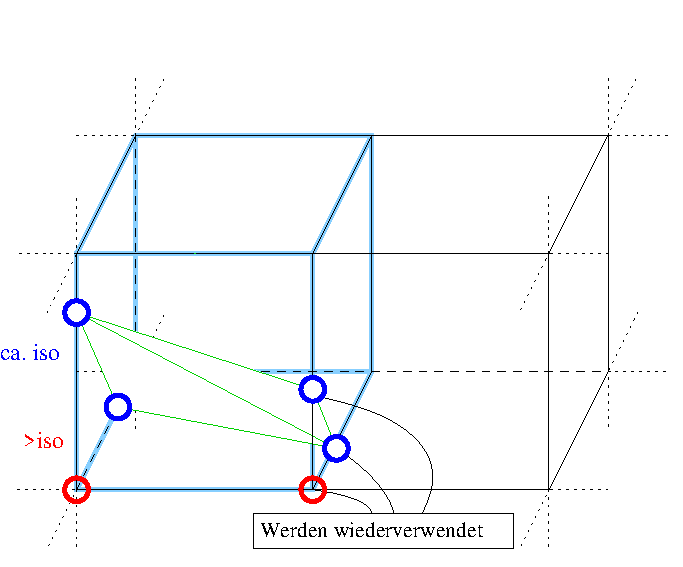
\includegraphics{pix/MC1.eps}
	\caption{Marching Cube auf einem regelm��igen Skalarfeld mit Knoten unterhalb eines Isowertes (rot), dadurch resultierenden Punkten auf den Kanten (blau) und der mit Hilfe einer Tabelle erzeugten zugeh�rigen Triangulierung (gr�n).}
	\label{fig:MC1}
	\end{center}
\end{figure}
F�r jeden W�rfel werden die Ecken bestimmt, die einen festen Isowert �berschreiten. Auf Kanten, die die Isofl�che durchdringen, da die beteiligten Ecken nicht beide ober- bzw. unterhalb des Isowertes liegen, wird mittels Interpolation bestimmt, an welcher Stelle der Isowert angenommen wird. Nun werden auf Grund der Eck-Konfiguration (einfacher Tabellenaufruf, siehe \cite{MC}) die ermittelten Punkte auf den Kanten zu einer Isofl�che des einzelnen W�rfels verbunden. Beim Durchlaufen des Skalarfeldes k�nnen die Daten des vorangegangenen W�rfels, also Skalarwerte an schon ausgewerteten Ecken und Kanten wiederverwendet werden. So marschiert also der W�rfel durch das Skalarfeld und erzeugt, unter der Annahme von Randpunkten des Skalarfeldes, die alle unterhalb des Isowertes liegen, eine geschlossene H�lle um alle Knoten, die oberhalb liegen. Die Vorschrift f�r die Triangulierung eines W�rfels ist damit noch nicht eindeutig. Siehe dazu Abb. \ref{fig:MC3}.
\begin{figure}[htb]
	\begin{center}
	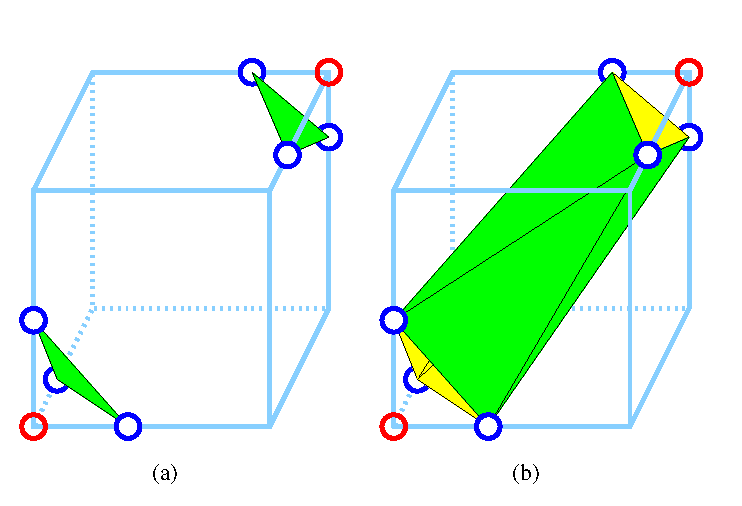
\includegraphics{pix/MC3.eps}
	\caption{Wahlfreiheit der Triangulierung}
	\label{fig:MC3}
	\end{center}
\end{figure}

Auf der Website \cite{MC} fand ich die Liste einer Beispielimplementierung des MCA. Diese habe ich, leicht abgewandelt, in meiner Arbeit verwendet. So stellte ich sicher, dass in Situationen wie in Abb. \ref{fig:MC3} stets Fall (a) gew�hlt wird, da ohnehin eines der st�rendsten Artefakte des Algorithmus {\em instabile}, durch Flackern auffallende Verbindungen zwischen einzelnen Tropfen oder Fl�ssigkeitsansammlungen sind.

Je n�her sich Partikel kommen m�ssen, um als eine Zusammenhangskomponente dargestellt zu werden, desto gr��er ist auch die Wahrscheinlichkeit, dass die Physik eine parallele Bewegung auf einer kritischen Distanz verhindert, welche besonders zu derartigen Artefakten f�hren d�rfte.

\paragraph{Bemerkung:} Da auch sehr nah benachbarte Partikel diagonal benachbart sein k�nnen, k�nnte diese These auch falsch sein. Generell ist aber eine Bewegung nahe dem Grenzfall zwischen {\em verbunden} und {\em nicht verbunden} nie auszuschlie�en.

Die Physik ist zwar wie in Kapitel \ref{KOL} gezeigt auf einem sehr gro�en Gebiet berechenbar. Nur leider liegt auf diese Weise nun auch kein f�r den MCA ben�tigtes Skalarfeld vor. Dieses auf dem gesamten Simulationsgebiet zu erzeugen w�rde wieder eingangs beschriebene Speichermengen verlangen.

\section{A grid to march on}
Um nun den MC loslaufen zu lassen, wird ein Gitter ben�tigt.
Genau genommen ben�tigt der MCA aber nur jene Gitterzellen, deren Ecken sowohl innerhalb, als auch au�erhalb der Fl�ssigkeit liegen.
Ein guter Anfang sind also jene Zellen, die �berhaupt Ecken in der Fl�ssigkeit haben.

\subsection{Ecken bestimmen}
\label{eckenbestimmen}
Der erste Schritt ist also die Bestimmung dieser Ecken (siehe Abb. \ref {fig:MCex01} auf Seite \pageref{fig:MCex01}).
Dazu verwendete ich eine Liste �hnlich der Listen, die f�r die Physik verwendet werden (siehe Kapitel \ref{verfeinertesgitter}). Nun wird der Zellindex aufeinanderfolgender Partikel verglichen und eine Liste angelegt, die jedem verwendeten Zellindex die Anzahl der darin befindlichen Partikel zuordnet. Auf diese Weise werden die Zellen der physikalischen Simulation zu den Ecken des MCA.

\paragraph{Bemerkung:}Die hier ebenfalls vorhandene Dichte $\rho$ der Partikel aufzusummieren hatte bei meinen Versuchen nur negative Effekte, sollte aber weiterhin in Betracht gezogen werden.

\subsection{Gitterzellen zu den Ecken}
\label{pendinglist}
Als n�chstes wird eine Liste der an die gefundenen Ecken angrenzenden W�rfel erzeugt. Da davon ausgegangen werden kann, dass der Zellindex der $i$-ten Ecke gr��er ist als der der ($i-1$)-ten, wurde der W�rfel, der von der $i$-ten Ecke und
\begin{equation*}
	\mbox{$i$-te Ecke + W�rfelgr��e} \cdot\left(\begin{matrix} 1 \\ 1 \\ 1 \end{matrix}\right)
\end{equation*}
aufgespannt wird, noch nicht erzeugt und kann so {\em ungepr�ft} als neuer W�rfel in eine W�rfelliste aufgenommen werden. Jeder andere an die $i$-te Ecke angrenzende W�rfel k�nnte bereits als solch ein {\em ungepr�ft aufgenommener} W�rfel in der Liste vorhanden sein.

\paragraph{Einschub:}Alle acht an die Ecke grenzenden W�rfel zu erzeugen und in eine Hashtable zu schreiben h�tte zwar �ber 1000 Zeilen Code sparen k�nnen, w�re aber sicher wesentlich langsamer, da mein Code die spezielle Struktur des Problems ausn�tzt.

Deshalb wird nun auch eine Liste von W�rfeln, "`pending\_cubes"', also "`anstehende W�rfel"' habe ich sie getauft, durchlaufen, deren Zellindex im letzten Durchlauf noch als potentieller Nachbarw�rfel eines noch kommenden neuen W�rfels in Frage kam. W�rfel, f�r die dies nicht mehr zutrifft, werden aus der pending\_list gel�scht. Wird ein Nachbarw�rfel gefunden
%\footnote{Da f�r manche Situationen die meisten Eintr�ge der pending\_list mit acht {\tt if}-Abfragen auf Nachbarschaft oder "`veraltet sein"' gepr�ft werden, ist ein Performancegewinn durch ein switch denkbar.}
, so wird die entsprechende Ecke des Nachbarw�rfels als der aktuellen Ecke zugeh�rig markiert. Wird einer der acht Nachbarw�rfel nicht gefunden, so wird dieser ebenfalls neu erzeugt. Alle neu erzeugten W�rfel werden in die pending\_list aufgenommen und es wird die n�chste Ecke abgearbeitet.
\begin{figure}[htbp]
	\begin{center}
	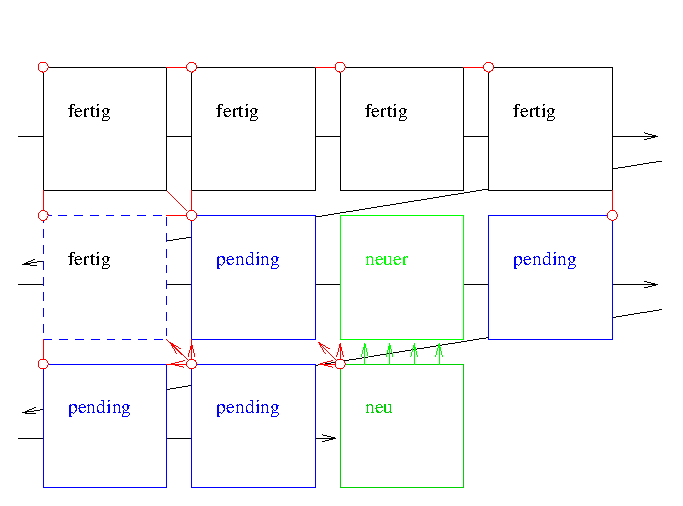
\includegraphics{pix/pendinglist01.eps}
	\caption{Bevor die Zelle "`neu"' in die Liste der Zellen aufgenommen wird, werden die Zellen "`pending"' auf Nachbarschaft gepr�ft und gemeinsame Punkte angepasst. Der ben�tigte Nachbar "`neuer"' fehlt noch und wird deshalb mit "`neu"' erzeugt und als "`pending"' in die Zellliste aufgenommen.}
	\label{fig:pendinglist01}
	\end{center}
\end{figure}

\paragraph{Bemerkung:} Da eine lange pending\_list potentiell zu einer in der Zellanzahl quadratischen Laufzeitordnung f�hrt, w�re es n�tig, die Zellsortierung f�r den MCA an die r�umliche Verteilung der Partikel zur Laufzeit anzupassen. Denkbar w�re hier etwa, die Koordinate, die die h�chsten Bits im Zellindex liefert, auszutauschen, sobald im letzten Bild die L�nge der pending\_list mehr als $\beta\%$ der Eckliste enthielt.

Abb. \ref{fig:pendinglist01} stellt zweidimensional die Entwicklung der W�rfelliste dar. Der dunkelgr�ne W�rfel wird in diesem Fall erzeugt, weil seine obere linke Ecke in der zuvor erzeugten Eckliste stand, also "`innerhalb der Fl�ssigkeit"' liegt. Beim Durchsuchen der pending\_list (blau) werden der linke Nachbar (Zellindex - 1) und der obere linke Nachbar (Zellindex - Zeilenl�nge - 1) gefunden und der erste W�rfel der zweiten Zeile (blau gestrichelt) aus der pending\_list entfernt. Bei den zwei gefundenen Nachbarn wird an der entsprechenden Ecke (rote Pfeile) der selbe Verweis auf die aktuelle Ecke gespeichert wie bei dem erzeugten W�rfel. Weil nach Durchlaufen der pending\_list feststeht, dass der obere Nachbar (hellgr�n) nie erzeugt wurde, wird er jetzt erzeugt und erh�lt die Eckinformation des aktuellen W�rfels. Die beiden gr�nen W�rfel werden der pending\_list angef�gt und es wird der n�chste Eckeintrag gelesen.

\subsection{Erzeugung der Oberfl�chenpunkte}

\paragraph{Bezeichnung:} Als Oberfl�chenpunkt bezeichne ich eine Ecke der gesuchten Oberfl�chentriangulierung. Als "`Vorw�rtsecke"' bezeichne ich die Ecke einer Zelle, die gem�� der Ecksortierung aus Kapitel \ref{eckenbestimmen} den h�chsten Index h�tte.

Die im letzten Abschnitt erzeugten W�rfel w�rden bereits f�r einen MCA gen�gen. Um allerdings die Oberfl�che wie in \ref{truform} beschrieben rund darstellen zu k�nnen, werden Normalen und damit auch weitere Informationen �ber die Umgebung der Oberfl�chenpunkte ben�tigt.\footnote{Das Deaktivieren der Normalenbestimmung w�rde die Oberfl�chenberechnung deutlich beschleunigen, ist aber nicht implementiert.}

Um Nachbarschaften auszuwerten, wird die eben ermittelte W�rfelliste sortiert und durchlaufen.
Als erstes werden, falls ben�tigt, die Oberfl�chenpunkte der drei Kanten erzeugt, welche an die "`Vorw�rtsecke"' angrenzen. Sie bekommen die Koordinate derjenigen benachbarten Ecke, die innerhalb der Fl�ssigkeit liegt (nur diese liegt explizit vor), plus einen Offset, der proportional zur dritten Wurzel der f�r diese Ecke gespeicherten Partikelanzahl ist und bereits berechnet vorliegt (Volumen $\propto$ Partikelanzahl $\propto$ Kantenl�nge$^3$). Die Koordinaten in der Liste der Ecken liegen nicht auf den Ecken des zugrunde liegenden regelm��igen Gitters. Siehe dazu Kapitel \ref{deformier}.

Mit dem Oberfl�chenvertex wird auch seine Normale in Abh�ngigkeit von der Eckkonfiguration des aktuellen W�rfels erzeugt.

\paragraph{Exkurs:} Auf welchen Kanten Oberfl�chenpunkte erzeugt werden m�ssen, h�ngt davon ab, welche Ecken innerhalb und welche au�erhalb der Fl�ssigkeit liegen. Da diese Information in meinem Programm als 8-Bit-Zahl, n�mlich ein Bit pro Ecke, vorliegt, �berlegte ich mir, hier an Stelle der sechs {\tt if}-Abfragen einen {\tt switch} auf besagte 8-Bit-Zahl durchzuf�hren. Diesen Programmteil schrieb ich mit Hilfe der {\tt if}-Abfragen automatisch. Daher sind diese knapp 4000 Zeilen Code auch in einer separaten Datei (siehe auch \ref{dateien}). Ist man nicht an Normalen interessiert, so sind von den 8 Bit nur 4 relevant und die Zeilenanzahl w�rde sich auf 90 reduzieren. Ich w�rde einen Performancegewinn erwarten, w�rde man genau diese Umwandlung vieler {\tt if}s in ein {\tt switch} auch bei der Auswertung der MC-Tabelle anwenden.

Nun wird, wieder mittels einer pending\_list (siehe Kapitel \ref{pendinglist}), die die Indizes der noch als Nachbarn in Frage kommenden Zellen h�lt, nach Nachbarn gesucht. Wird einer gefunden, so bekommt der aktuelle W�rfel an den sich ber�hrenden Kanten den Oberfl�chenpunktindex des Nachbarw�rfels �bertragen und die Normalen dieser Punkte werden mit der Eckkonfiguration des aktuellen W�rfels angepasst.
Auf diese Weise werden f�r jeden Oberfl�chenpunkt alle Ecken der 4 angrenzenden W�rfel ber�cksichtigt.

Die an und f�r sich falsche Annahme eines regelm��igen Gitters mit einer Dichte $\propto$ Partikelanzahl wird hier aus Performancegr�nden getroffen. Eine f�r korrekte Normalen ben�tigte Auswertung des auf den Partikeln gespeicherten Dichtefeldes findet nicht statt.

\subsection{Verbinden der Oberfl�chenpunkte}
In der W�rfelliste ist nun also sowohl die Eckkonfiguration gespeichert als auch alle relevanten Daten der Oberfl�chenpunkte. Die Information, welche drei Punkte jeweils zu einem Dreieck verbunden werden, wird nun wie in Kapitel \ref{MCA} aus einer Tabelle gelesen und als Triangulierungsliste gespeichert.

Die Triangulierungsliste ist mit der Liste der Oberfl�chenpunkte ausreichend, die MC-Oberfl�che darzustellen. Um zwischen benachbarten Dreiecken auch mit Lichtberechnung glatte �berg�nge zu erhalten ist die Liste der Normalen notwendig. Diese eignet sich aber auch, die Oberfl�che runder zu machen. Siehe dazu Kapitel \ref{truform}.

Abb. \ref{fig:MCex01}, \ref{fig:MCex02} und \ref{fig:MCex03} veranschaulichen nochmal in 2D die Vorgehensweise.
\begin{figure}[htbp]
	\begin{center}
	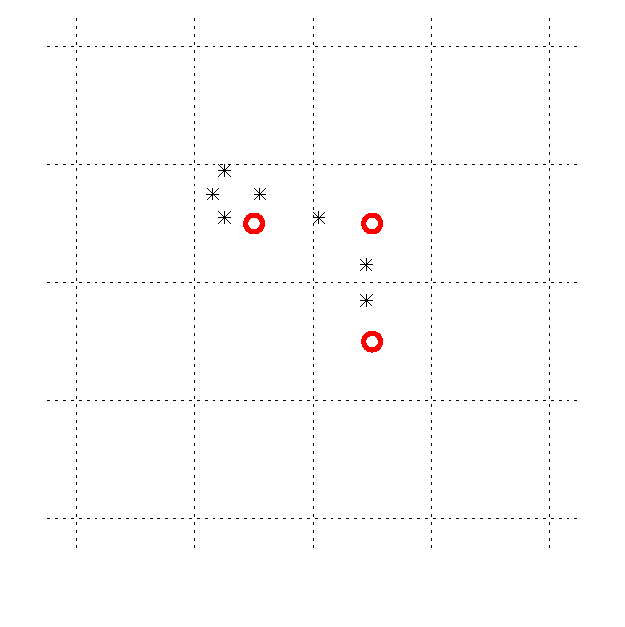
\includegraphics{pix/MCex01.eps}
	\caption{Die Anzahl der Partikel mit selbem Zellindex wird im Zellmittelpunkt als Ecke f�r den MCA gespeichert.}
	\label{fig:MCex01}
	\end{center}
\end{figure}
\begin{figure}[htbp]
	\begin{center}
	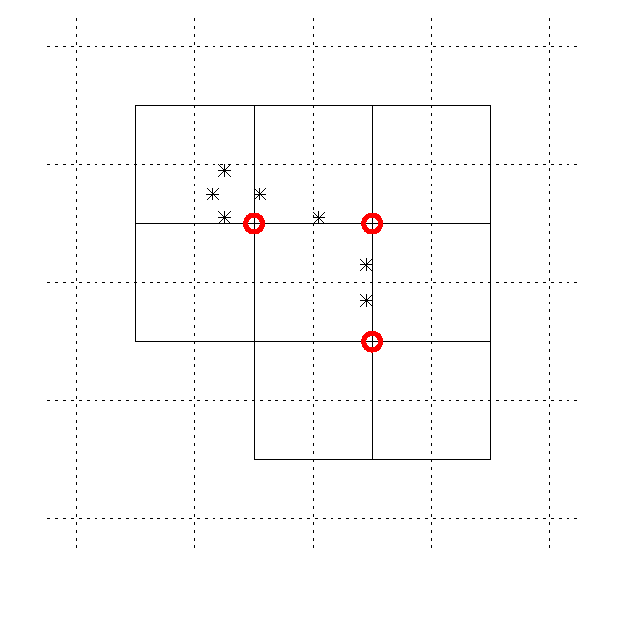
\includegraphics{pix/MCex02.eps}
	\caption{Alle Zellen mit Ecken {\em in der Fl�ssigkeit} werden erzeugt.}
	\label{fig:MCex02}
	\end{center}
\end{figure}
\begin{figure}[htbp]
	\begin{center}
	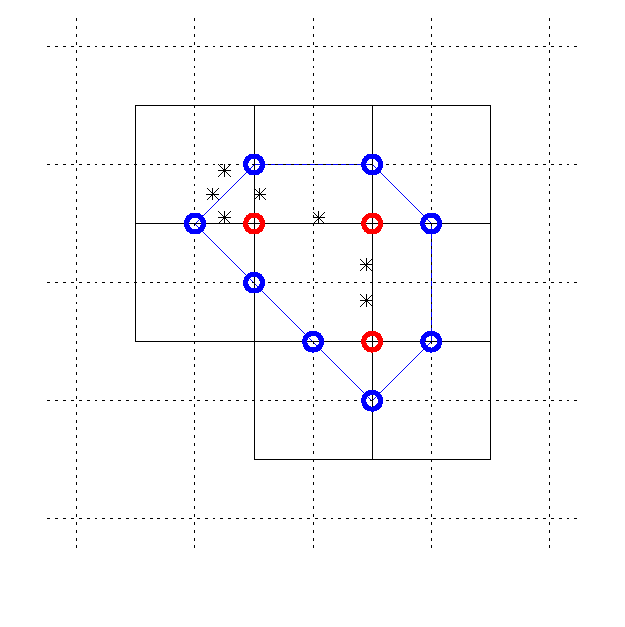
\includegraphics{pix/MCex03.eps}
	\caption{Punkte auf Kanten, die aus der Fl�ssigkeit herausf�hren, werden als Oberfl�chenpunkte markiert und verbunden.}
	\label{fig:MCex03}
	\end{center}
\end{figure}

\section{Deformiertes Gitter}
\label{deformier}
Ein weiterer Ansatz, die Oberfl�chentriangulierung n�her an die Partikel zu bringen, war es, beim Erzeugen der Ecken f�r den MCA auch die Schwerpunkte der Partikelpositionen an Stelle der Mittelpunktskoordinaten der Zellen zu speichern. Wie dann der MCA im Zweidimensionalen aussieht, veranschaulichen Abb. \ref{fig:MCex11}, \ref{fig:MCex12} und \ref{fig:MCex13}. Hier wurden die selben Partikelpositionen verwendet wie bei Abb. \ref{fig:MCex01}, \ref{fig:MCex02} und \ref{fig:MCex03}, S. \pageref{fig:MCex01}ff.
\begin{figure}[htbp]
	\begin{center}
	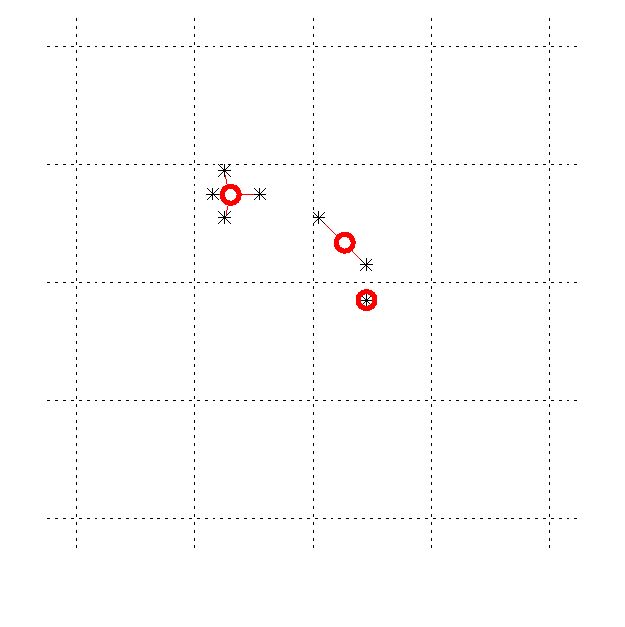
\includegraphics{pix/MCex11.eps}
	\caption{Schwerpunkt statt Zellmittelpunkt.}
	\label{fig:MCex11}
	\end{center}
\end{figure}
\begin{figure}[htbp]
	\begin{center}
	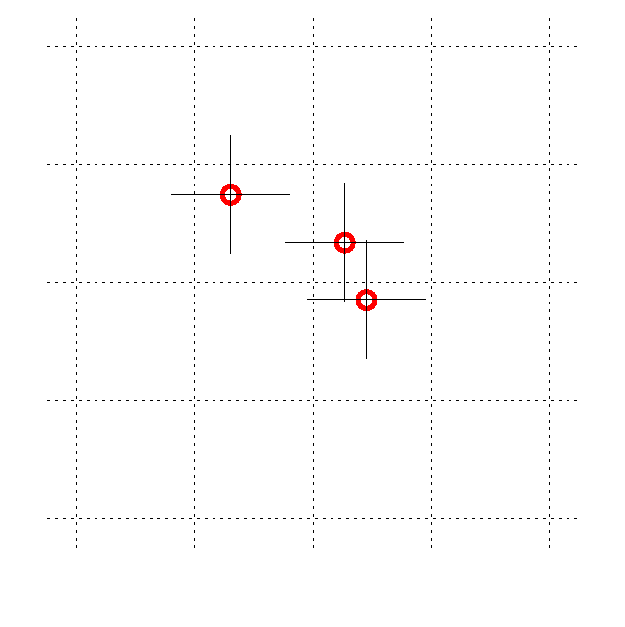
\includegraphics{pix/MCex12.eps}
	\caption{Die "`Ecken"' des Marching Cube "`Gitters"'.}
	\label{fig:MCex12}
	\end{center}
\end{figure}
\begin{figure}[htbp]
	\begin{center}
	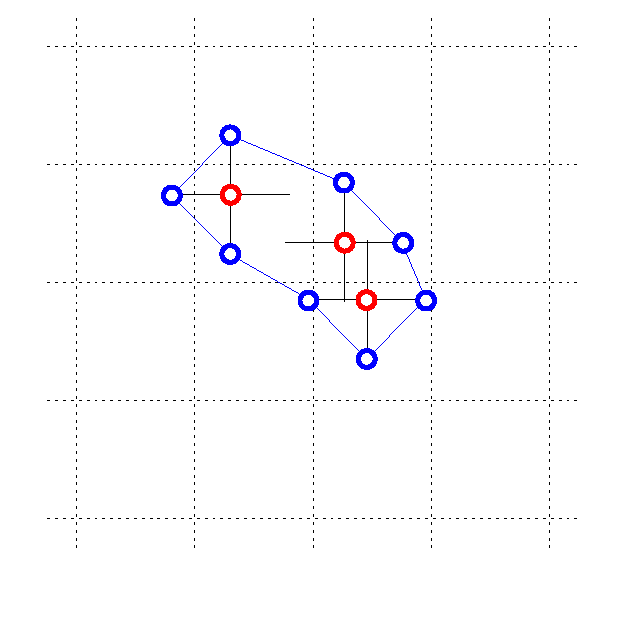
\includegraphics{pix/MCex13.eps}
	\caption{Eine nat�rlichere H�llkurve.}
	\label{fig:MCex13}
	\end{center}
\end{figure}

Ziel war es, das extrem st�rende Springen der Oberfl�che von einer Gitterposition zur n�chsten zu beseitigen. Das ist auch gelungen. Einzelnen Partikeln wird genau eine Ecke zugeordnet, die im Partikelmittelpunkt liegt und wenn sich der Index dieser Zelle �ndert sieht man das der Oberfl�che nicht an.

Mit dieser Modifikation kann es zur �berschneidung von H�llkurven kommen. Dies tritt verst�rkt dann auf, wenn bereits einzelne Partikel wie in Abb. \ref{fig:ueberschneid} (a) sehr gro� dargestellt werden.
\begin{figure}[htbp]
	\begin{center}
	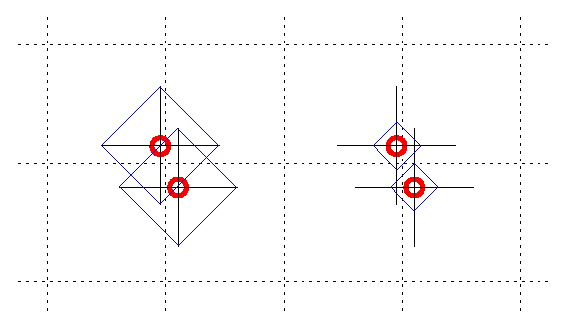
\includegraphics{pix/ueberschneid.eps}
	\caption{Verschieben des MC-Gitters kann zu �berschneidungen f�hren.}
	\label{fig:ueberschneid}
	\end{center}
\end{figure}
Gar wie in Abb. \ref{fig:entartet} (a) dargestellte entartete Fl�chen entstehen, wenn zugleich Fl�chen h�herer Ordnung (Kapitel \ref{truform}) verwendet werden und die Normalen ung�nstig bestimmt werden.
\begin{figure}[htbp]
	\begin{center}
	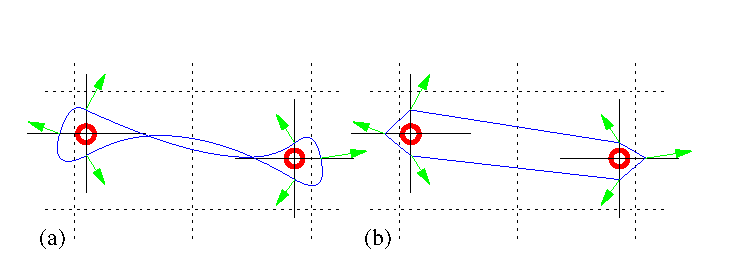
\includegraphics{pix/entartet.eps}
	\caption{Entartete Fl�chen bei schlecht gew�hlten Normalen.}
	\label{fig:entartet}
	\end{center}
\end{figure}
Beide Effekte fallen bei meiner Anwendung wahrscheinlich deshalb nicht ins Auge, weil mein Wasser nicht transparent ist.
\section{Fl�chen h�herer Ordnung}
\label{truform}
Die wie im letzten Kapitel erzeugte Oberfl�che ist sehr eckig. Ein einzelnes Partikel zum Beispiel wird als Oktaeder dargestellt, da nacheinander das Folgende erzeugt wird:
\begin{enumerate}
\item eine Ecke
\item acht W�rfel
\item sechs Oberfl�chenpunkte
\item acht Dreiecke
\end{enumerate}

W�nschenswert w�re aber eine Kugel, was in meiner Anwendung nicht ganz erreicht wird.
Ich suchte also einen Algorithmus, der Dreiecke anhand der Normaleninformation verfeinert, dabei aber jede Kante unabh�ngig von der dritten Ecke des Dreiecks unterteilt. Dies ist notwendig, will man die Verfeinerung ohne Nachbarschaftsinformationen durchf�hren. Dabei stie� ich auf ATIs TRUFORM-Erweiterung, die laut \cite{ATI} bereits 2001 mit der Radeon 2 Grafikkarte auf Hardware implementiert war.
Diese Erweiterung erzeugt Dreiecksgitter einer fest vorgegebenen Verfeinerungsstufe mit Gitterpunkten, die auf dem bikubischen Bezier-Patch liegen, das durch das Dreieck und seine Normalen definiert ist. Die Kanten von Bezier-Patches sind die zu den jeweiligen Ecken und ihren Normalen geh�renden Splinekurven. Damit h�ngt auch eine regelm��ige Unterteilung dieser Kanten nicht von der dritten Ecke ab und die TRUFORM-Fl�chen auf gleicher Stufe unterteilter benachbarter Dreiecke f�gen sich nahtlos aneinander.

Die Normalen der so erzeugten Dreiecke k�nnen wahlweise linear oder kubisch interpoliert sein. Warum lineare Interpolation nicht so gute Resultate liefert, soll Abb. \ref{fig:linkub} veranschaulichen. Andererseits ben�tigt die kubische Interpolation mehr Rechenzeit.

\begin{figure}[htbp]
	\begin{center}
	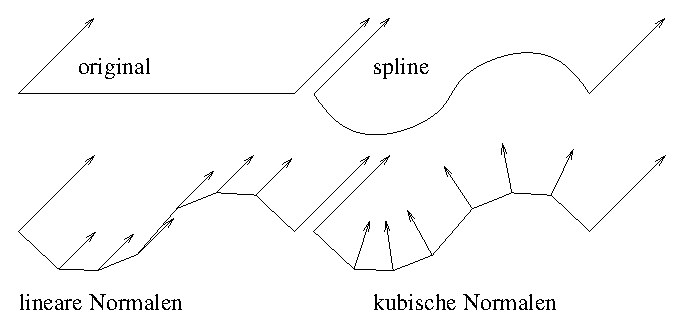
\includegraphics{pix/linkub.eps}
	\caption{Linear vs. kubisch interpolierte Normalen bei ATIs TRUFORM-Erweiterung.}
	\label{fig:linkub}
	\end{center}
\end{figure}
In meiner Implementierung schalte ich grunds�tzlich die Verfeinerung auf die maximale Stufe (7), da die Erzeugung der Oberfl�chendreiecke ohnehin weit mehr Zeit in Anspruch nimmt als die Unterteilung aller Dreiecke in 64 Teildreiecke durch eine ATI Radeon 9600. So l�uft meine Simulation in manchen F�llen (wenig Physik) mit 5.000 * 64 = 320.000 Dreiecken noch mit 30 Bildern pro Sekunde.

ATI TRUFORM$^\texttt{TM}$ zu verwenden, geht vorerst leider nur unter Windows. Dort erfordert es
unter DIRECT X und unter Open GL lediglich das Einbinden der ATI-header und Einschalten der Erweiterung.

\paragraph{Bemerkung:} Ein interessantes Thema ist die Frage, ob man �hnlich wie ATI TRUFORM Dreiecke auch mit unterschiedlichen Detailstufen effizient unterteilen kann. So k�nnte etwa f�r jede Dreiecksseite, die ja bei benachbarten Dreiecken �bereinstimmen, abh�ngig vom Viewport eine Unterteilungsstufe festgelegt werden, um anschlie�end das Dreieck zu unterteilen.

\section{Verfeinerung des Gitters}
\label{verfeinertesgitter}
In den meisten Anwendungen f�hrt ein verfeinertes Gitter f�r den MCA auch zu einer verbesserten Approximation der gesuchten Isofl�che.
Um zu testen, ob bei meinem Verfahren auch eine Verbesserung zu erzielen ist, f�hrte ich zu den vier sortierten Listen der Partikel (siehe Kapitel \ref{KOL}) eine F�nfte ein, die nach einem Gitter mit halber Maschenweite sortiert war.

Da aber der ab Kapitel \ref{eckenbestimmen} beschriebene Ansatz jedes Partikel nur einer Ecke zuordnet und kein H�henfeld um Partikel ausgewertet wird, zeigte die Verfeinerung des Gitters keine signifikante Verbesserung des Ergebnisses. Die Artefakte wurden zwar kleiner, aber wahrscheinlich auch h�ufiger. Eventuell hat die Verfeinerung den positiven Effekt, dass Partikel seltener verbunden dargestellt werden, solange ihr Abstand zueinander gr��er ist als der Interaktionsradius.
	\chapter{Anwendung}
\label{anwendung}
\section{Systemvoraussetzungen}
Die folgenden Voraussetzungen gelten f�r die Beispielimplementierung. Selbstverst�ndlich kann zur Visualisierung auch jede andere Software verwendet werden, wodurch evtl. mehr RAM oder eine einfachere Grafikkarte ben�tigt w�rde. Die {\tt Fluid} Klasse liefert Rohdaten, die auf verschiedenste Weise aufbereitet werden k�nnen.
\begin{itemize}
	\item {Betriebssystem}\\
		Die Quelldateien zu dieser Diplomarbeit wurden sowohl unter Windows-XP, als auch unter Linux (Debian \& SuSE) compiliert.
		Da von ATI f�r Linux keine Treiber f�r deren TRUFORMs zur Verf�gung standen, sind TRUFORMs unter Linux per Default deaktiviert.
	\item {RAM}\\
		Je nach Partikelanzahl (Abh�ngig von der Fl�che der Kontrollpolygone und dem Volumen des Fluids) k�nnen 15MB freier Speicher ausreichen.
		Ein Testlauf mit 380000 Partikeln ergab einen Speicherbedarf von unter 130MB.
	\item {Grafikkarte}\\
		Zur Visualisierung empfiehlt sich eine ATI-Karte ab Radeon 9600, da diese TRUFORMs unterst�tzt.
		Leider existieren daf�r aber wie gesagt nur Windows-Treiber.
	\item {weitere Software}\\
		OpenGL, GLUT und ATIExtensions m�ssen f�r die Beispielimplementierung vorhanden sein.
\end{itemize}

\section{Ben�tigte Dateien}
\label{dateien}
\begin{itemize}
	\item {Fluid.h}\\
		Diese Datei enth�lt die Klasse {\tt Fluid} mit den in (\ref{member}) beschriebenen Methoden, die zur blo�en Anwendung
		meiner Ergebnisse ausreichend sind. Der Versuch, die Particleengine von der Physik und Visualisierung
		der Partikel als Fl�ssigkeit zu trennen gelang leider nicht, da mein Ansatz zur Visualisierung
		die Strukturen der Physik-Engine verwendet und damit alles in einer Klasse besser aufgehoben ist.
	\item {autogenerated.h}\\
		Diese Datei resultierte aus dem Versuch, die Performance zu steigern, indem geschachtelte {\tt if}s
		durch ein switch ersetzt werden. Der Erfolg war zwar minimal, aber doch messbar. Somit findet sich
		in Fluid.h an entsprechender Stelle ein {\tt \#include} \"{\tt autogenerated.h}\".
	\item {Particle.h}\\
		Diese Datei enth�lt die Klasse {\tt Particle}. {\tt Particle}s speichern ihre Koordinate, Geschwindigkeit, Beschleunigung, Dichte, Informationen, ob sie Kontrollpartikel (siehe \ref{Kontrollpartikel}) sind, ihre Indizes in den vier sortierten Listen und in welcher der vier Listen sie komplett in einer Zelle Liegen.
	\item {Vektor.h}\\
		Diese Datei enth�lt die Klasse {\tt Vektor}. Eine Instanz von {\tt Vektor} ist ein Vektor im dreidimensionalen euklidischen Vektorraum. Die Klasse unterst�tzt unter anderem Addition ({\tt operator+(Vektor)}), Kreuzprodukt ({\tt operator\%(Vektor)}), Skalarprodukt ({\tt operator*(Vektor)}), Vektorprodukt ({\tt operator*(float), operator/(float)}), L�ngennormierung ({\tt norm(float)}) und Ermittlung der L�nge ({\tt abs()}).
\end{itemize}
\section{Notation}
Um Feldvariablen leserlich darzustellen, sind im Folgenden beispielsweise {\tt float-}Werte zu Gruppen zusammengefasst dargestellt, die im Feld keine eigenen Untereinheiten darstellen.
${\tt float *feld} = \{\vec{a}_1,\vec{a}_2,\vec{a}_3\}, \vec{a}_i=\{a_i^x, a_i^y\}$
hei�t
${\tt float *feld} = \{a_1^x,a_1^y,a_2^x,a_2^y,a_3^x,a_3^y\}$. $\{\}$ steht hier �brigens nicht
f�r die mathematische Mengenklammer, sondern stellt eine C$^{++}$ Feldzuweisung dar.
\section{Public member von {\tt Fluid}}
\label{member}
Die Fluidsimulation wurde in C$^{++}$ realisiert und kann durch Verwendung der Klasse
{\tt Fluid} in Projekten verwendet werden. {\tt Fluid} besitzt die folgenden "offentlichen
member-Funktionen:
\subsection{Konstruktor}
Die Klasse {\tt Fluid} enth�lt nur einen Konstruktor

{\tt Fluid::Fluid(const long maxparticlecount,\\
const float particlesize,\\
const float ax, const float ay, const float az,\\
const float minx, const float miny, const float minz,\\
const float maxx, const float maxy, const float maxz)}

\begin{itemize}
	\item {{\tt const long maxparticlecount}}\\
		Gibt die maximale Anzahl an zu verwendenden Partikeln an. Dies bezieht
		sich sowohl auf Kontrollpartikel, als auch auf die Fluid-Partikel. Ist
		{\tt maxparticlecount} keine Zweierpotenz, so wird die n�chst h�here
		Zweierpotenz verwendet. Ein �berschreiten dieser Limitierung im sp�teren
		Programmablauf f�hrt zu einem Abbruch!
	\item {{\tt const float particlesize}}\\
		Gibt die Granularit�t an. Je kleiner die Partikel, desto mehr werden pro
		Volumen Fl�ssigkeit ben�tigt. Es werden auch mehr Kontrollpartikel ben�tigt.
	\item {{\tt const float ax, const float ay, const float az}}\\
		Eine globale Beschleunigung. In der Regel die Gravitation.
	\item {{\tt const float minx, const float miny, const float minz}}\\
		Minimale Koordinate des Simulationsbereichs.
	\item {{\tt const float maxx, const float maxy, const float maxz}}\\
		Maximale Koordinate des Simulationsbereichs. Wird vergr��ert auf das n�chstgr��ere
		${\tt max}={\tt min}+2^n*{\tt cellsize}={\tt min}+2^n*4*{\tt particlesize}$
\end{itemize}

Auch wenn im hier verwendeten Verfahren die Kollisionsdetektion nicht mittels
Expliziter Speicherung aller Zellen realisiert wird, ergibt sich doch eine
Obergrenze bez�glich Partikelanzahl und Simulationsgebiet.
Mit einer Zellgr��e von ${\tt cellsize}=4*{\tt particlesize}$ ergibt sich eine Unterteilung in\\
${\tt cells_x}=({\tt maxx}-{\tt minx})/{\tt cellsize}$\\
${\tt cells_y}=({\tt maxy}-{\tt miny})/{\tt cellsize}$\\
${\tt cells_z}=({\tt maxz}-{\tt minz})/{\tt cellsize}$.\\
$\log_2({\tt maxparticlecount})+\log_2({\tt cells_x})+\log_2({\tt cells_y})+\log_2({\tt cells_z})+3$
mu� $\leq 64$ sein.



\subsection{trianglelist2boundary}
\label{trianglelist2boundary}

{\tt void Fluid::trianglelist2boundary(float * trianglelist, unsigned int firsttriangleid, unsigned int lasttriangleid)}

Mit dieser Funktion werden lokale Grenzfl�chen definiert. Die Grenzbedingung wirkt sich {\tt particlesize} bis $\sqrt{41}*${\tt particlesize} �ber die Dreiecksr�nder hinaus aus, wodurch Dreiecke sich ungewollt �berlappen k�nnen. Partikel, die sich von der {\em aktiven} Seite dem Dreieck n�hern, werden auf die {\em erlaubte} Seite verschoben.
Deshalb ist zu beachten, W�nde mit gen�gend Abstand, also mindestens $6.5*${\tt particlesize} anzuordnen.

Der Rechenaufwand ist nicht proportional zur Anzahl der Dreiecke, sondern zur Fl�che der Dreiecke, da diese mit virtuellen Begrenzungspartikeln �berzogen werden.
Diese Begrenzungspartikel z�hlen zum {\tt maxparticlecount}, sind aber bei weitem nicht so zeitraubend in der Berechnung, wie die bewegten Partikel, die die Fl�ssigkeit darstellen.

N�here Informationen zu Kontrollpartikeln finden sich auch in Kapitel \ref{Kontrollpartikel}.

\begin{itemize}
	\item {{\tt float * trianglelist}}\\
		Liste von Dreieckskoordinaten in der Form
		\begin{eqnarray*}
			{\tt * trianglelist} & = & \{Dreieck_0, Dreieck_1, \cdots, Dreieck_n\}\\
			Dreieck_i & = & \{\vec{x}_i^0, \vec{x}_i^1, \vec{x}_i^2\}\\
			\vec{x}_i^j & = & \{x_i^j, y_i^j, z_i^j\}\\
			0\le i \le n & \wedge & 0 \le j \le 2
		\end{eqnarray*}
		Die {\em erlaubte} Seite ist die, in die $(\vec{x}_i^1-\vec{x}_i^0) \times (\vec{x}_i^2-\vec{x}_i^0)$ zeigt.
	\item {{\tt unsigned int firsttriangleid, unsigned int lasttriangleid}}\\
		Die Liste von Dreieckskoordinaten wird nur von $Dreieck_{\tt firsttriangleid}$ bis $Dreieck_{\tt lasttriangleid}$
		verwendet.\\ $0 \le {\tt firsttriangleid} < {\tt lasttriangleid} \le n$
\end{itemize}

\subsection{trianglelist2teleport}
\label{trianglelist2teleport}

{\tt void Fluid::trianglelist2teleport(float target\_x, float target\_y, float target\_z, float * trianglelist, unsigned int firsttriangleid, unsigned int lasttriangleid)}

Wie bei {\tt trianglelist2boundary} (\ref{trianglelist2boundary}) wird auch bei {\tt trianglelist2teleport} eine Grenzfl�"-che definiert, bei deren �berschreiten eine Aktion ausgef�hrt wird. Die Partikel werden zu der Koordinate {\tt (target\_x, target\_y, target\_z)}$^T$ "`teleportiert"'. Das hei�t, sie werden an den Ort {\tt (target\_x, target\_y, target\_z)}$^T+\vec{\delta}$ verschoben. $\vec{\delta}$ verhindert dabei, dass mehrere Partikel, die im gleichen Zeitschritt zum selben Ort teleportiert wurden exakt die selbe Koordinate erhalten. Generell ist aber zu beachten, da� ein Teleport evtl. viele Partikel an einen Ort zusammenf�hrt und ist deshalb entweder mit einem SetSpeed (\ref{trianglelist2setspeed}) zu kombinieren, indem eine SetSpeed-Fl�che an der Zielkoordinaten initialisiert wird, oder der Teleport wird durch ein Shift (\ref{trianglelist2shift}) ersetzt, welcher nicht zu Instabilit�ten f�hrt, solange im Zielgebiet kein starker Stau entsteht.

N�here Informationen zu Kontrollpartikeln finden sich auch in Kapitel \ref{Kontrollpartikel}.

\begin{itemize}
	\item {{\tt float target\_x, float target\_y, float target\_z}}\\
		Die Koordinate, zu der die Fl�ssigkeit teleportiert werden soll.
	\item {{\tt float * trianglelist}}\\
		Liste von Dreieckskoordinaten wie bei {\tt trianglelist2boundary} (\ref{trianglelist2boundary})
	\item {{\tt unsigned int firsttriangleid, unsigned int lasttriangleid}}\\
		Die Liste von Dreieckskoordinaten wird nur von $Dreieck_{\tt firsttriangleid}$ bis $Dreieck_{\tt lasttriangleid}$
		verwendet.\\
		$0 \le {\tt firsttriangleid} < {\tt lasttriangleid} \le n$
\end{itemize}

\subsection{trianglelist2shift}
\label{trianglelist2shift}

{\tt void Fluid::trianglelist2shift(float shift\_x, float shift\_y, float shift\_z, float * trianglelist, unsigned int firsttriangleid, unsigned int lasttriangleid)}

�hnlich wie bei {\tt trianglelist2teleport} (\ref{trianglelist2teleport}) wird hier jedes Fluidpartikel, das mit einem der Begrenzungsdreiecke kollidiert, d.h. in dessen aktiven Bereich gelangt, im Raum verschoben.
Da das Ziel dieser Verschiebung aber eine echte Ausdehnung hat, und zwar die Selbe wie ihr Ursprung, kommt es hier nicht allein aus der Verschiebung zu Instabilit�t, solange die Fl�ssigkeit am Ziel z�gig abflie�en kann.
Die Idee hinter dieser Funktion ist, dass Fl�ssigkeit, die sich im Innern eines Rohres befindet, nicht berechnet werden mu�. Liegt das Ziel dieses Shifts allerdings in einem Bereich, wo die Fl�ssigkeit nicht von alleine abflie�t, wird auch hier ein SetSpeed (\ref{trianglelist2setspeed}) ben�tigt, um zu vermeiden, da� Fl�ssigkeitspartikel an die Position anderer Partikel verschoben werden.

N�here Informationen zu Kontrollpartikeln finden sich auch in Kapitel \ref{Kontrollpartikel}.

\begin{itemize}
	\item {{\tt float shift\_x, float shift\_y, float shift\_z}}\\
		({\tt shift\_x, shift\_y, shift\_z})$^T$ ist der Vektor, um den die Fl�ssigkeit verschoben werden soll.
	\item {{\tt float * trianglelist}}\\
		Liste von Dreieckskoordinaten wie bei {\tt trianglelist2boundary} (\ref{trianglelist2boundary})
	\item {{\tt unsigned int firsttriangleid, unsigned int lasttriangleid}}\\
		Die Liste von Dreieckskoordinaten wird nur von $Dreieck_{\tt firsttriangleid}$ bis $Dreieck_{\tt lasttriangleid}$ verwendet.\\
		$0 \le {\tt firsttriangleid} < {\tt lasttriangleid} \le n$
\end{itemize}

\subsection{trianglelist2setspeed}
\label{trianglelist2setspeed}

{\tt void Fluid::trianglelist2setspeed(float speed\_x, float speed\_y, float speed\_z, float * trianglelist, unsigned int firsttriangleid, unsigned int lasttriangleid)}

Um an machen Stellen Instabilit�ten zu vermeiden, ist es n�tig, die Fl�ssigkeit k�nstlich zu bewegen. Dies ist zum Beispiel der Fall im Zielbereich von {\tt trianglelist2teleport} (\ref{trianglelist2teleport}). {\tt trianglelist2setspeed} l�sst sich aber auch dazu verwenden, an beliebigen Stellen im Simulationsgebiet Str�mungen zu erzeugen.

N�here Informationen zu Kontrollpartikeln finden sich auch in Kapitel \ref{Kontrollpartikel}.

\begin{itemize}
	\item {{\tt float speed\_x, float speed\_y, float speed\_z}}\\
		({\tt speed\_x, speed\_y, speed\_z})$^T$ gibt die Geschwindigkeit f�r Partikel an, die auf die "`aktive"' Seite der Begrenzungsfl�che gelangen.
	\item {{\tt float * trianglelist}}\\
		Liste von Dreieckskoordinaten wie bei {\tt trianglelist2boundary} (\ref{trianglelist2boundary}).
	\item {{\tt unsigned int firsttriangleid, unsigned int lasttriangleid}}\\
		Die Liste von Dreieckskoordinaten wird nur von $Dreieck_{\tt firsttriangleid}$ bis $Dreieck_{\tt lasttriangleid}$ verwendet.\\
		$0 \le {\tt firsttriangleid} < {\tt lasttriangleid} \le n$
\end{itemize}

\subsection{tetraederlist2liquid}

{\tt void Fluid::tetraederlist2liquid(float * tetraederlist, unsigned int firsttetraid, unsigned int lasttetraid)}

Mit dieser Funktion werden Fluidvolumina definiert.
Die �bergebenen Tetraeder werden mit Fluidpartikeln gef�llt.
Dabei kann es zu einem Abbruch kommen, wenn der zuvor definiert Wert f�r {\tt maxparticlecount} zu niedrig ist.

\begin{itemize}
	\item {{\tt float * tetraederlist}}\\
		Liste von Tetraederkoordinaten in der Form
		\begin{eqnarray*}
			{\tt * tetraederlist} & = & \{Tetraeder_0, Tetraeder_1,\cdots,Tetraeder_n\}\\
			Tetraeder_i & = & \{\vec{x}_i^0,\vec{x}_i^1,\vec{x}_i^2,\vec{x}_i^3\}\\
			\vec{x}_i^j & = & \{x_i^j,y_i^j,z_i^j\}\\
			0\le i \le n & \wedge & 0 \le j \le 3
		\end{eqnarray*}
		Die Reihenfolge der Tetraederecken spielt hier keine Rolle.
	\item {{\tt unsigned int firsttetraid, unsigned int lasttetraid}}\\
		Die Liste von Tetraederkoordinaten wird nur von $Tetraeder_{\tt firsttetraid}$ bis $Tetraeder_{\tt lasttetraid}$
		verwendet.
\end{itemize}

\subsection{progress}

{\tt int Fluid::progress(const float dt)}

Mit dieser Funktion wird der Zustand nach der �bergebenen Zeit {\tt dt} berechnet.
Von {\tt dt} h�ngt ma�geblich das Verhalten der Fl�ssigkeit ab.
Bei zu gro�en Zeitschritten kommen numerische Instabilit�ten zum Tragen.
Au�erdem k�nnen evtl. lokale Begrenzungen �bersprungen werden.
Der R�ckgabewert gibt an, ob eine neue Position der Partikel berechnet wurde (1) oder nicht (0).

\subsection{movingparticlecount}

{\tt unsigned long Fluid::movingparticlecount(void)}

Diese Funktion gibt die Anzahl aller Partikel zur�ck, die die Fl�ssigkeit darstellen.

\subsection{boundaryparticlecount}

{\tt unsigned long Fluid::boundaryparticlecount(void)}

Diese Funktion gibt die Anzahl aller Partikel zur�ck, die f�r Kontrollmechanismen wie Grenzl�chen (\ref{trianglelist2boundary}), Teleporter (\ref{trianglelist2teleport}), Shifter (\ref{trianglelist2shift}) und SetSpeed-Fl�chen (\ref{trianglelist2setspeed}) verwendet wurden.

\subsection{particlecount}

{\tt unsigned long Fluid::particlecount(void)}

Diese Funktion gibt die Anzahl aller Partikel ({\tt movingparticlecount()} + {\tt boundaryparticlecount()}) zur�ck.

\subsection{get\_particlearray}

{\tt void Fluid::get\_particlearray(float ** VertexArray, unsigned long \& arraylength)}

Liefert die Positionen aller Partikel. Die ersten {\tt movingparticlecount()} Koordinaten sind Fl�ssigkeitspartikel, die {\tt boundaryparticlecount()} folgenden sind Koordinaten von Kontrollpartikeln.

\begin{itemize}
	\item {{\tt float ** VertexArray}}\\
		Dies ist ein Zeiger auf ein Feld von Koordinaten der Form
		\begin{eqnarray*}
			* VertexArray & = & \{\vec{x}_0,\vec{x}_1,\cdots,\vec{x}_n\}\\
			\vec{x}_i & = & \{x_i,y_i,z_i\}\\
		\end{eqnarray*}
		verwendet den bereits reservierten Speicherbereich, falls {\tt arraylength} ausreichend gro� ist. Ansonsten wird der Speicherbereich freigegeben und ein neuer der L�nge $3*{\tt particlecount}$ reserviert.
	\item {{\tt unsigned long \& arraylength}}\\
		Sollte mindestens $3*{\tt particlecount}$ sein und wird wie eben beschrieben verwendet, um die Gr��e des Feldes gegebenenfalls anzupassen. Dieser Wert enth�lt nach Aufruf von {\tt get\_particlearray} \underline{\em nicht} die Anzahl der geschriebenen Werte!
\end{itemize}

\subsection{get\_surfacegrid}

{\tt int Fluid::get\_surfacegrid(float ** VertexArrayPointer, float ** NormalArrayPointer, unsigned long \& vn\_arraylength, unsigned long \& vn\_count, unsigned long ** triangleindicesPointer, unsigned long \& ti\_arraylength)}


\begin{itemize}
	\item {{\tt float ** VertexArrayPointer, float ** NormalArrayPointer, unsigned long \& vn\_arraylength}}\\
		Die zwei {\tt ArrayPointer} funktionieren mit {\tt vn\_arraylength} genauso, wie {\tt VertexArray} und {\tt arraylength} in der Methode {\tt get\_particlearray(float ** VertexArray, unsigned long \& arraylength)}. {\tt float ** VertexArrayPointer} ist dabei ein Zeiger auf das Feld der Ecken der Oberfl�che der Fl�ssigkeit, {\tt float ** NormalArrayPointer} ein Zeiger auf das Feld der zugeh�rigen Normalen.
		\begin{eqnarray*}
			{\tt * VertexArrayPointer} & = & \{\vec{v}_0,\vec{v}_1,\cdots,\vec{v}_{vn\_count-1}\}\\
			\vec{v}_i & = & \{v^x_i,v^y_i,v^z_i\}\\
			{\tt * NormalArrayPointer} & = & \{\vec{n}_0,\vec{n}_1,\cdots,\vec{n}_{vn\_count-1}\}\\
			\vec{n}_i & = & \{n^x_i,n^y_i,n^z_i\}\\
		\end{eqnarray*}
	\item {{\tt unsigned long \& vn\_count}}\\
		Gibt an, wieviele der {\tt vn\_arraylength} Feldelemente neu geschrieben und somit relevant sind.
	\item {{\tt unsigned long ** triangleindicesPointer}}\\
		\label{triangleindicesPointer}
		Gibt an, welches Dreieck mit welchem Vertex inzidiert.
		\begin{eqnarray*}
			&{\tt *}& {\tt triangleindicesPointer}\\
			& = & \{ Dreieck_0,Dreieck_1,\cdots,Dreieck_{n-1}\}\\
			Dreieck_i & = &\{\vec{x}_i^0, \vec{x}_i^1, \vec{x}_i^2\}\\
			\vec{x}_i^j & = &\{x_i^j, y_i^j, z_i^j\}\\
		\end{eqnarray*}
		$n$ is der R�ckgabewert von {\tt get\_surfacegrid}
	\item {{\tt unsigned long \& ti\_arraylength}}\\
		Gibt an, wieviel Platz f�r {\tt * triangleindicesPointer} reserviert wurde und wird gegebenenfalls erh�ht.
	\item {R�ckgabewert {\tt int get\_surfacegrid}}\\
		Der R�ckgabewert ist die Anzahl der erzeugten Dreiecke.
\end{itemize}

\subsection{set\_height\_function}
\label{setheightfunction}

{\tt void Fluid::set\_height\_function(float (*height\_function)(float x, float y))}

Erm�glicht es, der Fl�ssigkeit ein auf dem ganzen Simulationsgebiet (global) g�ltiges H�henfeld zu �bergeben. Diese Funktion sollte
mit geringstm�glichem Zeitaufwand auszuwerten sein,
da jedes bewegte Partikel in jedem Zeitschritt gegen dieses H�henfeld auf G�ltigkeit gepr�ft wird.
Im Einzelfall ist zu �berlegen, ob lokale Begrenzungen mittels {\tt trianglelist2boundary} (\ref{trianglelist2boundary}) nicht performanter sind, als ein kompliziertes H�henfeld.

\begin{itemize}
	\item {{\tt float (*height\_function)(float x, float y))}}\\
		Ist der Zeiger auf eine Funktion {\tt float height\_function(float, float)}.
\end{itemize}

\subsection{set\_height\_function\_normal}

{\tt void Fluid::set\_height\_function\_normal(Vektor (*height\_function\_normal)(float x, float y))}

\begin{itemize}
	\item {{\tt Vektor (*height\_function\_normal)(float x, float y)}}\\
		Ist der Zeiger auf die Funktion\\
		{\tt Vektor height\_function\_normal(float, float)}. Diese
		sollte die nicht normierte Normale der Funktion, die {\tt set\_height\_function} (\ref{setheightfunction}) �bergeben
		wurde, zur�ckgeben. Falsche Normalen, z.B. mit negativer $z$-Komponente k�nnen zu unerwartetem Verhalten, bis hin zum Absturz der Software f�hren. Andererseits k�nnen mit Normalen, die nicht zur {\tt set\_height\_function} �bergebenen Funktion passen evtl. erw�nschte Effekte oder Vereinfachungen erzielt werden.
\end{itemize}

\subsection{height\_function}

{\tt float Fluid::height\_function(float x, float y)}

Gibt den Wert des H�henfeldes bei $(x,y)$ zur�ck.

\subsection{height\_function\_normal}

{\tt Vektor Fluid::height\_function\_normal(float x, float y)}

Gibt die Normalenrichtung des globalen H�henfeldes bei $(x, y)$ zur�ck. Die Normale hat eine positive $z$-Komponente.

\subsection{minxyz}

{\tt Vektor Fluid::minxyz(void)}

Gibt die minimale Ecke {\tt Vektor}$(min_x, min_y, min_z)$ des Simulationsgebiets zur�ck.

\subsection{maxxyz}

{\tt Vektor Fluid::maxxyz(void)}

Gibt die maximale Ecke {\tt Vektor}$(max_x, max_y, max_z)$ des Simulationsgebiets zur�ck.

\subsection{particleradius}

{\tt float Fluid::particleradius(void)}

Gibt den Partikelradius zur�ck. Das ist der maximale Abstand bei dem Partikel interagieren k�nnen. Kontrollpartikel wirken sich auf die gesamte Zelle in der sie sich befinden aus. Somit ist ihr Effekt nicht auf {\tt particleradius} beschr�nkt, sondern geht deutlich dar�ber hinaus.

\section{Die Beispielimplementierung}

Mit Hilfe der auf der beiliegenden CD enthaltenen Visual Studio Projekt Datei bzw. f�r Linux dem ebenfalls enthaltenen Makefile
l�sst sich meine Beispielimplementierung kompilieren und ausf�hren.

\subsection{Programmstart}
Dieses Programm initialisiert eine Fl�ssigkeit als ein Tetraedervolumen, darunter einen Trichter aus Wanddreiecken, eine Shiftfl�che am unteren Ende des Trichters welche die Fl�ssigkeit um die halbe H�he zwischen Trichter und Nullpunkt transportiert, einen SetSpeed Bereich, der die Fl�ssigkeit in positiver x-Richtung bewegt wo die Fl�ssigkeit zuletzt noch auf eine Teleportfl�che trifft, die sie wieder nach weit oberhalb des Trichters bef�rdert.

Die Simulation startet im Pausemodus. Mausbewegungen rotieren die Szene um den Koordinatendreifu� im Nullpunkt, welcher in etwa die Mitte der Szene ist. Das Rechte-Maustaste-Men� ist selbsterkl�rend.
\subsection{Tastaturbelegung}
Mit Hilfe der Tastatur k�nnen einige Simulations- und Visualisierungsparameter ver�ndert werden.

%\begin{tabular}{crl}
\begin{center}
\begin{tabular}{|l|l|p{8cm}|}
\hline
Taste 	& Effekt			& Bemerkung\\
\hline
\hline
ESC		& Ende				& Beendet das Programm.\\
p		& Pause				& Schaltet die Physik, nicht aber \newline die Oberfl�chenermittlung an/aus.\\
*, /	& Geschwindigkeit 	& Ver�ndern die Simulationsgeschwindigkeit um $\pm$10\%.\\
+, -	& Zoom				& �ndern die Distanz zum Zentrum um 20\%\\
c		& Oberfl�che		& Schaltet die Berechnung/Darstellung der Fl�ssigkeitsoberfl�che an/aus.\\
t		& TRUFORM			& Schaltet ATI TRUFORM an/aus. (nur bei Windows)\\
n		& Normalen			& Schaltet die Fluidnormalen an/aus falls die Fl�ssigkeitsoberfl�che
							  visualisiert wird, denn nur dann werden Normalen berechnet.\\
f		& flat				& Schaltet das Shading auf "`flat"'. Nurnoch eine Farbe pro Dreieck.\\
g		& smooth			& Schaltet das Shading auf "`smooth"'. Farbe des Dreiecks wird zwischen den Ecken interpoliert.\\
y		& Volumen			& Gibt das von der Fl�ssigkeitsoberfl�che umh�llte Volumen auf die Konsole aus.\\
v		& Partikel			& Schaltet die Partikeldarstellung an/aus.\\
l		& Licht				& Schaltet die Beleuchtung an/aus.\\
e		& filled			& Schaltet die Vorderseiten auf "`ausgef�llt"'.\\
w		& wireframe			& Schaltet die Darstellung auf "`nur Kanten"'.\\
q		& dots				& Schaltet die Darstellung auf "`nur Punkte"'.\\
TAB		& 					& Schaltet die R�ckseiten auf transparent.\\
\hline
\end{tabular}
\end{center}
	\chapter{Resultate}
\label{resultate}
Wie schon an verschiedenen Stellen in dieser Diplomarbeit erw�hnt, sind mit den vorgestellten Verfahren Partikelsimulationen mit minimalem Speicherbedarf m�glich. Laut Windows Taskmanager ben�tigt die Simulation, aus der die folgenden Screenshots stammen, bei 830 dargestellten und 4000 f�r die Physik verwendeten Partikeln f�r die Physik und die Oberfl�chenberechnung gemeinsam unter 20MB. Dabei h�ngt der Speicherbedarf linear von der Partikelanzahl, der Anzahl der Oberfl�chenpunkte und der Anzahl der Zellen, die Fl�ssigkeit enthalten, ab.

Die Bildwiederholfrequenz liegt bei dieser Simulation auf einem Athlon 1.2GHz PC mit ATI Radeon 9600 zwischen 16 und 70 Bildern pro Sekunde.

Die Bilder in diesem Kapitel sind meist Stereoskopien, also Bilder der selben Szene aus leicht variierten Blickwinkeln.
Betrachtet man diese Bilder, indem man versucht, hindurch zu blicken, so erfasst das linke Auge das linke Bild und das rechte Auge das rechte Bild und es entsteht ein dreidimensionaler Eindruck. Um das Fokussieren zu erleichtern, ist eine m�glichst helle Beleuchtung hilfreich.

Auf diese Weise kann schon bei der Punktewolke in Bild \ref{fig:ss7fit} die r�umliche Verteilung dieser Punkte erfasst werden. Diese Punkte sind die Zentren der Partikel, auf denen die Physik simuliert wird.
\begin{figure}[htb]
	\begin{center}
	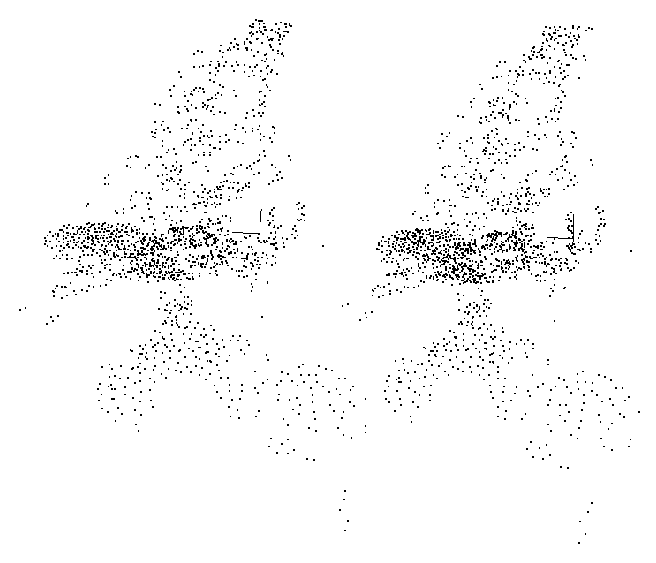
\includegraphics{pix/ss7fit.eps}
	\caption{Partikel einer Fl�ssigkeit, die auf eine Ebene str�mt.}
	\label{fig:ss7fit}
	\end{center}
\end{figure}

In Bild \ref{fig:ss6} wird die selbe Punktverteilung, allerdings mit den Verfahren aus Kapitel \ref{vis}, dargestellt. Die Oberfl�che ist rund und wirkt organisch.
\begin{figure}[htb]
	\begin{center}
	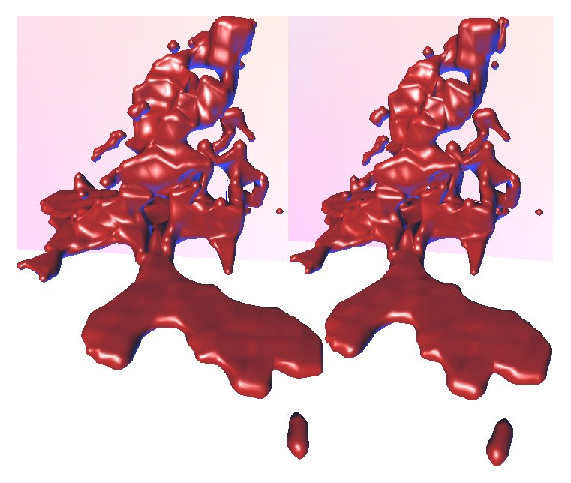
\includegraphics{pix/ss6.eps}
	\caption{Die Oberfl�chendarstellung zur Partikelverteilung aus Abb. \ref{fig:ss7fit}.}
	\label{fig:ss6}
	\end{center}
\end{figure}

Ohne Abrunden der Oberfl�che sieht man allerdings sofort, dass das Gitter des Marching Cube Algorithmus sehr grob ist (siehe Abb. \ref{fig:3d4}). Tropfen erscheinen als Oktaeder, die Lichtquellen erzeugen keine Spiegellinien.
\begin{figure}[htb]
	\begin{center}
	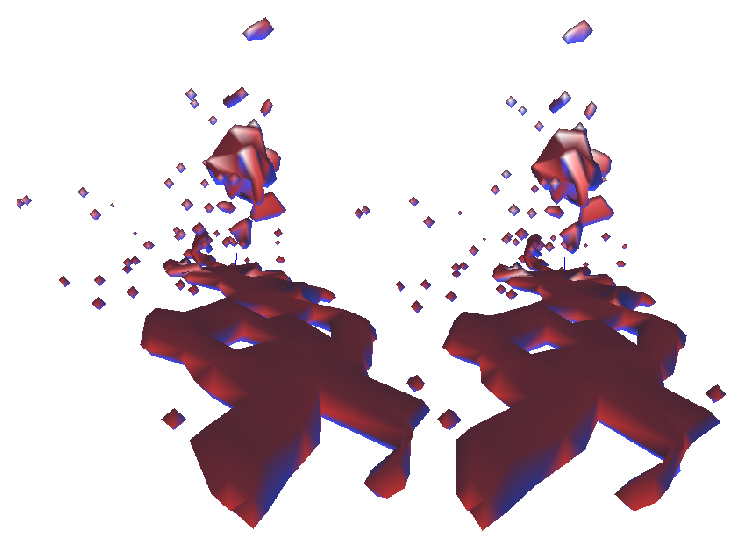
\includegraphics{pix/3d4.eps}
	\caption{Ohne ATI-TRUFORM wirkt alles eckig und man sieht keine Spiegellinien.}
	\label{fig:3d4}
	\end{center}
\end{figure}

Dass die wie in Abb. \ref{fig:ueberschneid} (a) auf Seite \pageref{fig:ueberschneid} dargestellte �berschneidung von Fl�chen auch tats�chlich beobachtet werden kann, zeigt Bild \ref{fig:ss8}. Entartungen, wie in Bild \ref{fig:entartet} (a) beschrieben, sind mir seit der Verfeinerung des Gitters nicht mehr aufgefallen.
\begin{figure}[htb]
	\begin{center}
	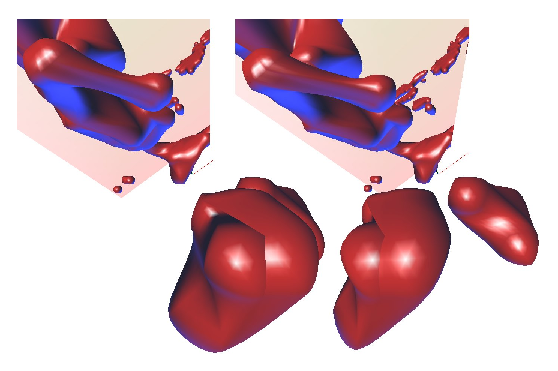
\includegraphics{pix/ss8.eps}
	\caption{Selbst�berschneidung der Oberfl�che.}
	\label{fig:ss8}
	\end{center}
\end{figure}

In Abb. \ref{fig:spritzwasser} verteilen sich Partikel auf einem gro�en Gebiet. Gerade in Szenen, in denen nicht viele Partikel interagieren, ist die Bildrate besonders hoch. Auch wenn hier ca. 5.000\footnote{5.000 mal 64 wegen der ATI-TRUFORMs.} Dreiecke die Oberfl�che darstellen, werden noch �ber 35 Bilder pro Sekunde erreicht. Die Oberfl�chenberechnung wird nur dann langsam, wenn sich viel Oberfl�che auf der selben $z$-Koordinate befindet.
\begin{figure}[htb]
	\begin{center}
	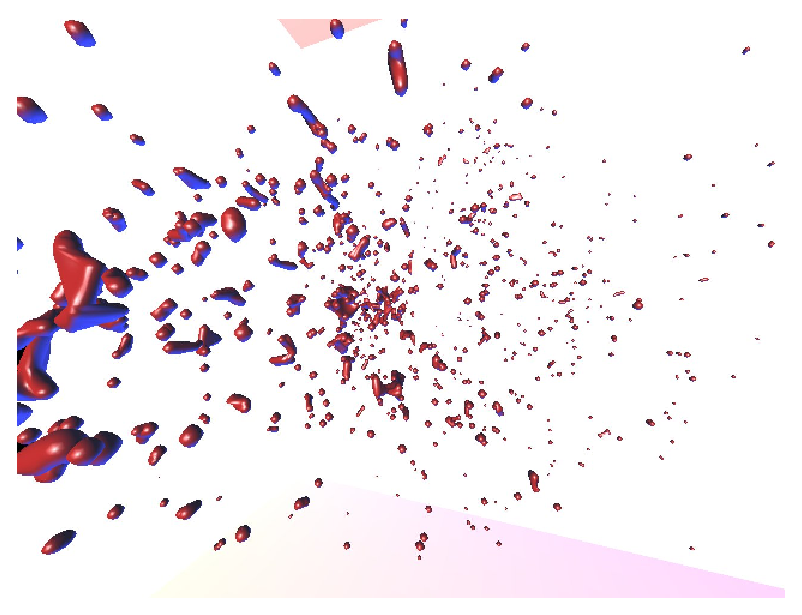
\includegraphics{pix/spritzwasser.eps}
	\caption{Spritzeffekt.}
	\label{fig:spritzwasser}
	\end{center}
\end{figure}
\chapter{Ausblick}
\label{ausblick}
Auch wenn die hier gezeigten Resultate noch nicht nach Wasser aussehen, denke ich, dass schon bald erste Anwendungen entwickelt werden, die vielleicht nur kleine Mengen Wasser, oder zumindest nicht-transparente Fl�ssigkeiten, in interaktiven Umgebungen integriert zeigen werden.

Obwohl das Trennen und Vereinen von Tropfen mit meinem Marching-Cube-Algorithmus unsch�ne Artefakte erzeugt, kann er eventuell in modifizierter Form, insbesondere mit einem besseren Algorithmus zur Bestimmung der Normalen als schnelle Methode zur Erzeugung runder H�llfl�chen weiter Anwendung finden.

Ver�nderungen, die n�tig w�ren, um Fl�ssigkeiten verschiedener physikalischer Eigenschaften zu simulieren stehen in keinem Widerspruch zu den vorgestellten Methoden. Im Gegenteil. So wie die Kontrollpartikel nur in der Physik von den Fl�ssigkeitspartikeln unterschieden werden, k�nnten auch, theoretisch beliebig viele, verschiedene Fl�ssigkeiten miteinander interagieren.

\chapter{Danksagung}

Abschlie�end m�chte ich mich bei den Mitarbeitern des Lehrstuhls f�r Computer Graphik \& Visualisierung der TU M�nchen, insbesondere Herr Prof. Dr. Westermann, sowie bei Prof. Dr. Huckle bedanken, dass sie meine Diplomarbeit in dieser Form m�glich gemacht haben. Aber auch Freunde und Familie die mir mit Rat und Tat zur Seite standen m�chte ich danken.

	\begin{center}
		\begin{picture}(300,80)
			%\put(0,0){\framebox(300,80){}}
			%\graphpaper[10](0,0)(300,80)
			\qbezier(70,45)(40,45)(40,30)
			\qbezier(40,30)(40,15)(80,15)
			\qbezier(80,15)(100,15)(150,30)
			\qbezier(150,30)(200,45),(220,45)
			\qbezier(220,45)(260,45),(260,30)
			\qbezier(260,30)(260,15),(230,15)
		\end{picture}
	\end{center}

	\begin{thebibliography}{66}
		\bibitem{FOFE} Nick Foster \& Ronald Fedkiw:\\
		\newblock {\em "`Practical animation of liquids"'},\\
		\newblock Proceedings of ACM SIGGRAPH 2001.

		\bibitem{ETHZ} Matthias M"uller, David Charypar \& Markus Gross:\\
		\newblock {\em "`Particle-Based Fluid Simulation for Interactive Applications"'},\\
		\newblock Department Institute of Technology Z"urich (ETHZ), Schweiz, 2003.

		\bibitem{MC} Paul Bourke:\\
		\newblock {\em "`Polygonising a scalar field"'},\\
		\newblock http://astronomy.swin.edu.au/pbourke/modelling/polygonise/, 2003.

		\bibitem{ATI} http://www.ati.com

		\bibitem{NSG} http://scienceworld.wolfram.com/physics/Navier-StokesEquations.html

		\bibitem{UTAH} Simon Premo\v{z}e, Tolga Tasdizen, James Bigler, Aaron Lefohn \& Ross T. Whitaker:\\
		\newblock {\em "`Particle-Based Simulation of Fluids"'},\\
		\newblock University of Utah, 2003.

		\bibitem{SPH} Olaf Kessel-Deynet:\\
		\newblock {\em "`Ber�cksichtigung ionisierender Strahlung im Smoothed-Particle-Hydrodynamics-Verfahren und Anwendung auf die Dynamik von Wolkenkernen im Strahlungsfeld massiver Sterne"'},\\
		\newblock Ruprecht-Karls-Universit�t Heidelberg, 1999.
	\end{thebibliography}
	\addcontentsline{toc}{chapter}{Literaturverzeichnis}
	%*******************************************************************
	% Abbildungsverzeichnis
	%*******************************************************************
	%\addcontentsline{toc}{chapter}{Abbildungsverzeichnis}
	%\listoffigures
	%\cleardoublepage

%	\bibliography{bib.bib}   % verwendete bib-Dateien fuer die
 % \bibliography{Literatur}       % Generierung des Literaturverzeichnisses
\end{document}

%%%%%%%%%%%%%%%%%%%%%%%%%%%%%%%%%%%%%%%%%%%%%%%%%%%%%%%%%%%%%%%%%%%%%%%%%%%%%%
